\section{General Architecture of a Photonic Time-Stretch Data Acquisition System}
In this section, a general architecture of a Photonic Time-Stretch \gls{daq} is described. Such a system consists of a photonic front-end, which covers the time-stretching method and conversion of photons into electrical values. The general theory of the time-stretching technique is given, together with some basics about photodetectors. 

Furthermore, such a system contains an \gls{adc} which converts the analog values into digital signals that can be processed by a computing unit. A short overview of the basic \gls{adc}-theory is given, as well as of the most prominent figures of merit. Knowledge and understanding of these is necessary to define and/or evaluate the overall performance of the converter. 

Last but not least a \gls{daq} needs an appropriate computing system for collection, processing and visualization of the acquired data. As this part is use-case specific, there doesn't exist a general "theory" which can be described.

\subsection{Photonic Time-Stretch Front-End}
The working principle of the optic time-stretch technique can be described in two steps (see \autoref{fig:eo_ts}).
First, a short laser pulse (duration typically hundreds of femtoseconds) is propagated in a dispersive medium, e.g. an optical fiber of length $L_1$ (see \autoref{fig:eo_ts}). 
This results in a chirped laser pulse of the duration
\begin{equation}
	T_1 = \Delta \lambda D_1 L_1
\end{equation}
with the optical bandwidth of the laser pulse $\Delta \lambda$  and the dispersion parameter $D_1$ of the fiber.

The next step is the time-to-wavelength-mapping, where a temporal intensity modulation is imprinted on the chirped pulse. In this step, the laser pulse co-propagates with another pulse, e.g. \gls{thz} pulse from \gls{csr} (duration in the range of picoseconds), in an \gls{eo} crystal. Due to the Pockels effect\footnote{The Pockels effect describes the phenomenon of occurring and change of existing birefringence in an electric field, which is linearly proportional to the electric field strength." \cite{pockels}} the \gls{thz} pulse causes a time-dependent birefringence in the crystal.
This modulates the polarization of the laser pulse.

After that, the modulated chirped pulse propagates through another dispersive medium, a fiber of the length $L_2$.
In this way, the temporal modulation of the pulse is further stretched to the duration $T_2$, which is long enough for detection with photodetectors and/or digitizing with \Glspl{adc}. \cite{roussel2014}

The factor, by which the pulse is slowed down, is calculated as
\begin{equation}
	M = 1 + \frac{L_1}{L_2}.
\end{equation}

\begin{figure}[tbh]
	\centering
	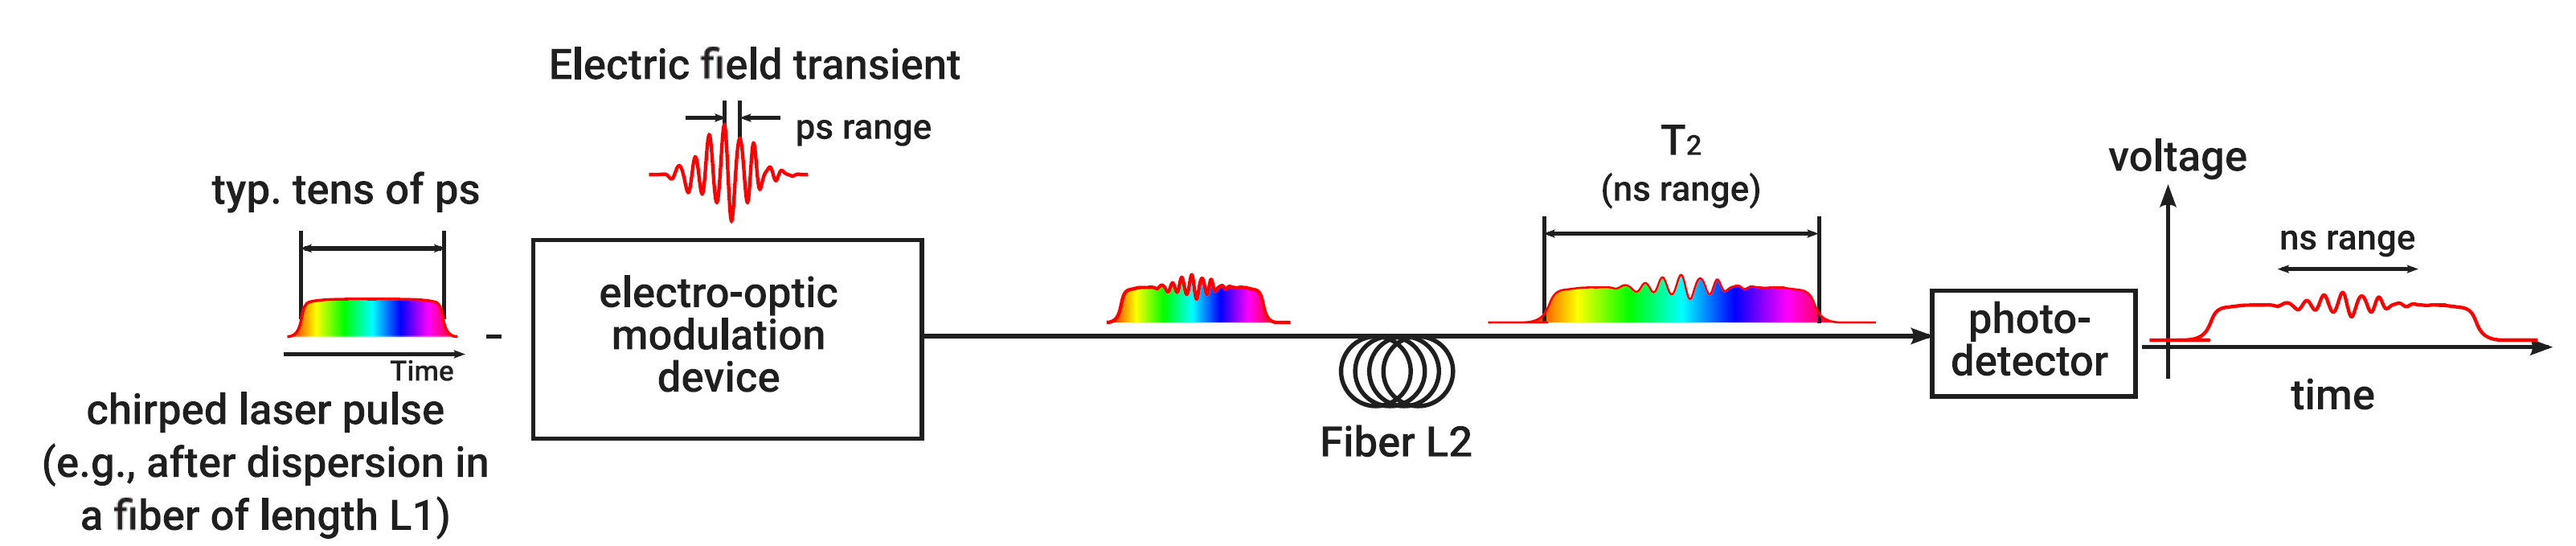
\includegraphics[width = \textwidth]{chap/02-theory/img/time_stretch.png}
	\caption{Electro-Optical Time-Stretch Technique \cite{szwaj}}
	\label{fig:eo_ts}
\end{figure}
%todo at least re-add labels in the figure with tikz, or they are too small


\paragraph{Detector/Diode}
A photodetector converts the incoming optical signal into an electrical signal, known as O/E convertor.
The detection and subtraction between the two stretched signals is performed using a amplified balanced photodetector (photoreceiver) from Discovery Semiconductors, with 20 GHz bandwidth and 2800 V/W gain (specified at 1500 nm). The two differential outputs of the detector are sent on a Lecroy LabMaster 10i oscilloscope with 36 GHz bandwidth, 80 GS/s sample rate on each channel and a memory of 256 Mega samples.

\subsection{Analog-To-Digital Converter}
\Glspl{adc} are used to translate analog voltages into digital signals, which can be processed by information processing, computing, data transmission and control systems. The translation can be seen as encoding a continuous-time analog input (voltage) into a series of discrete, $N$-bit words. This process, which is also called \textit{sampling}, can be expressed as
\begin{equation}
	V_{\text{In}} = V_{\text{FS}} \sum_{k = 0}^{N-1} \frac{b_k}{2^{k+1}} + \epsilon
\end{equation}
with $V_{\text{In}}$ being the input voltage, $V_{\text{FS}}$ the full-scale voltage, $b_k$ the individual output bits and $\epsilon$ the quantization error (described in \autoref{par:quant_noise}). \autoref{fig:idealADC} shows the ideal transfer function of a 3-bit \gls{adc}. As one can see, each digital $N$-bit word corresponds to a range of input voltage values (\textit{code width}), which is centered around a \textit{code center}. The input voltage is resolved to the code of the nearest code center.
\begin{figure}[H]
	\centering
	\includegraphics[width = 0.55\textwidth]{chap/02-theory/img/ideal_adc}
	\caption[Transfer function of ideal, 3-bit ADC]{Transfer function of an ideal, 3-bit \gls{adc} (redrawn from \cite{Lundberg})}
	\label{fig:idealADC}
\end{figure}


\subsubsection*{Sampling Theory}
An \gls{adc} samples an analog signal with a sample frequency $f_s$.
This frequency has to be chosen in such way, that the original signal can be fully reconstructed.
The \textit{Nyquist criteria} states, that in order to accurately represent a band-limited, continuous signal %todo what is B?
%todo rewrite the condition, maybe like 
\begin{equation}
	y (t) \, \fourier  Y(f) \quad \text{with} \quad Y(f)=0\vert_{f>B/2}
\end{equation}
it has to be sampled with a frequency $f_s$ respecting
\begin{equation}
	f_s > B \quad \text{or} \quad f_s > 2 f_a
\end{equation}
with $f_a$ being the highest frequency contained in the signal. \cite{walt,puente2015}
%todo why not relate f_a to B?

Violation of this rule leads to \textit{aliasing}.
%todo explain aliasing


\begin{figure}[tbh]
	\centering
	\begin{subfigure}{\textwidth}
		\centering
		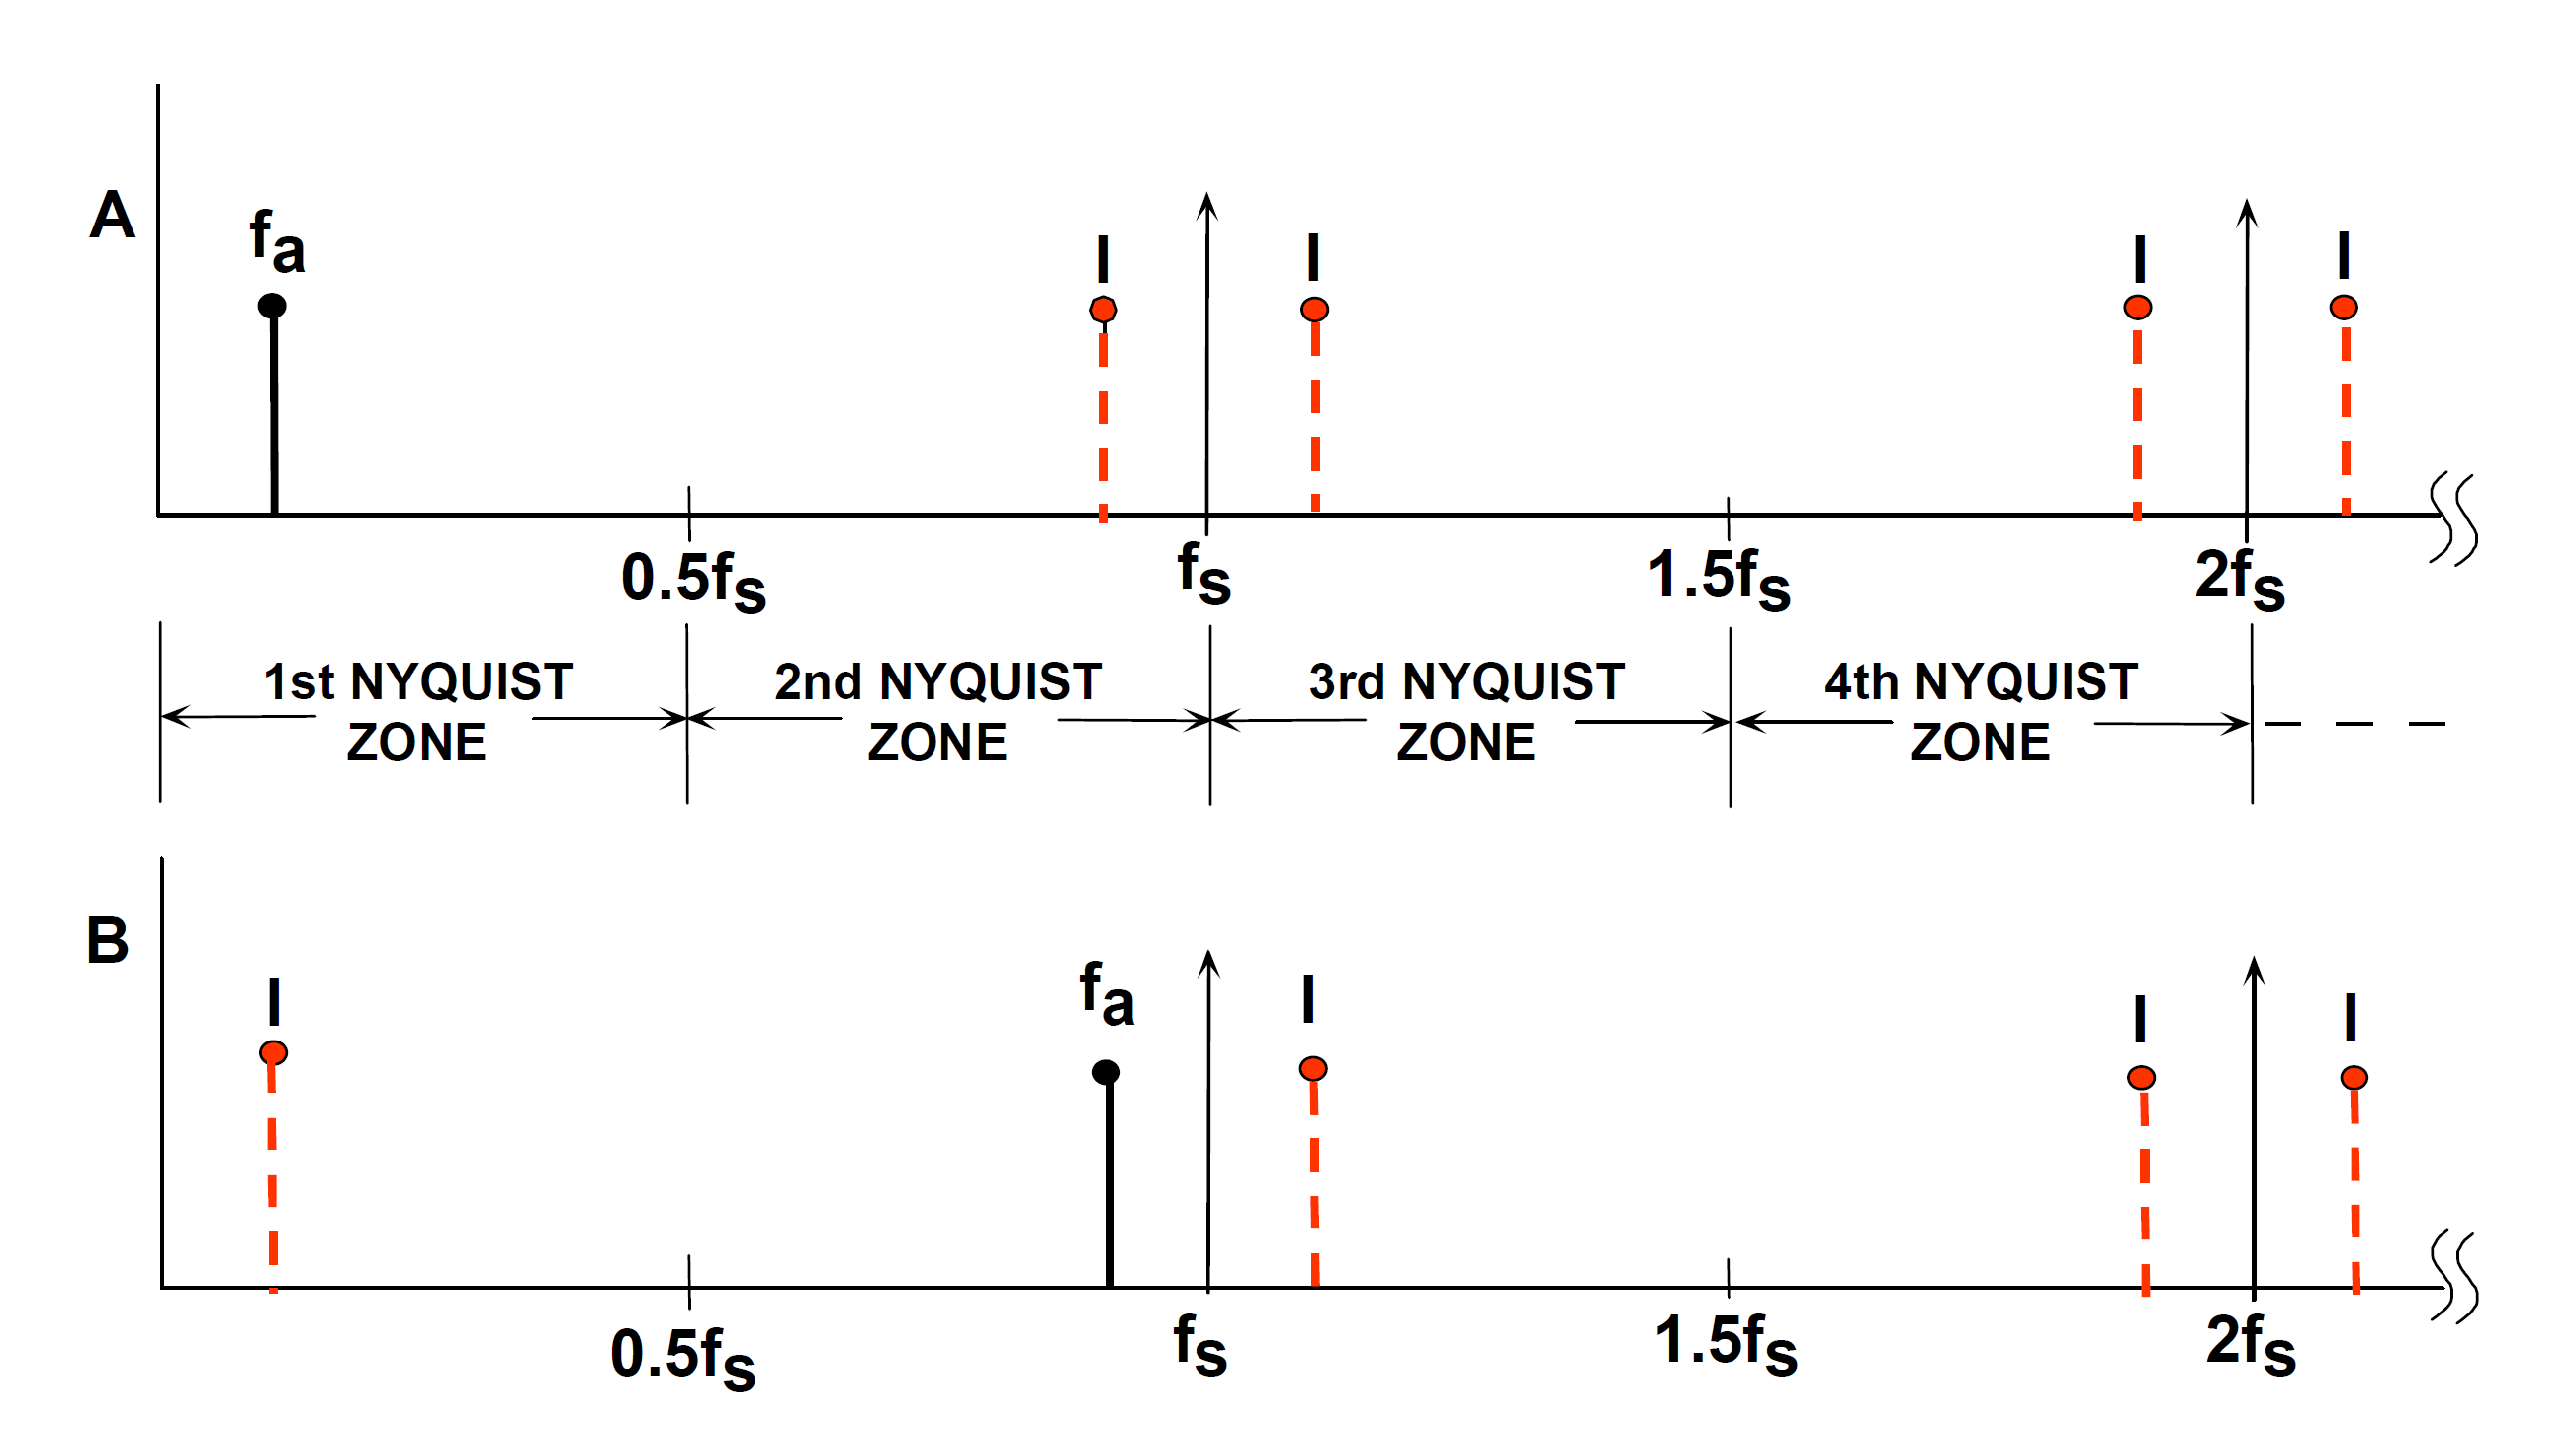
\includegraphics[width=\linewidth]{chap/02-theory/img/alias_f}  
		\caption{Sampling in frequency domain}
		\label{fig:alias_f}
	\end{subfigure}
	\begin{subfigure}{\textwidth}
		\centering
		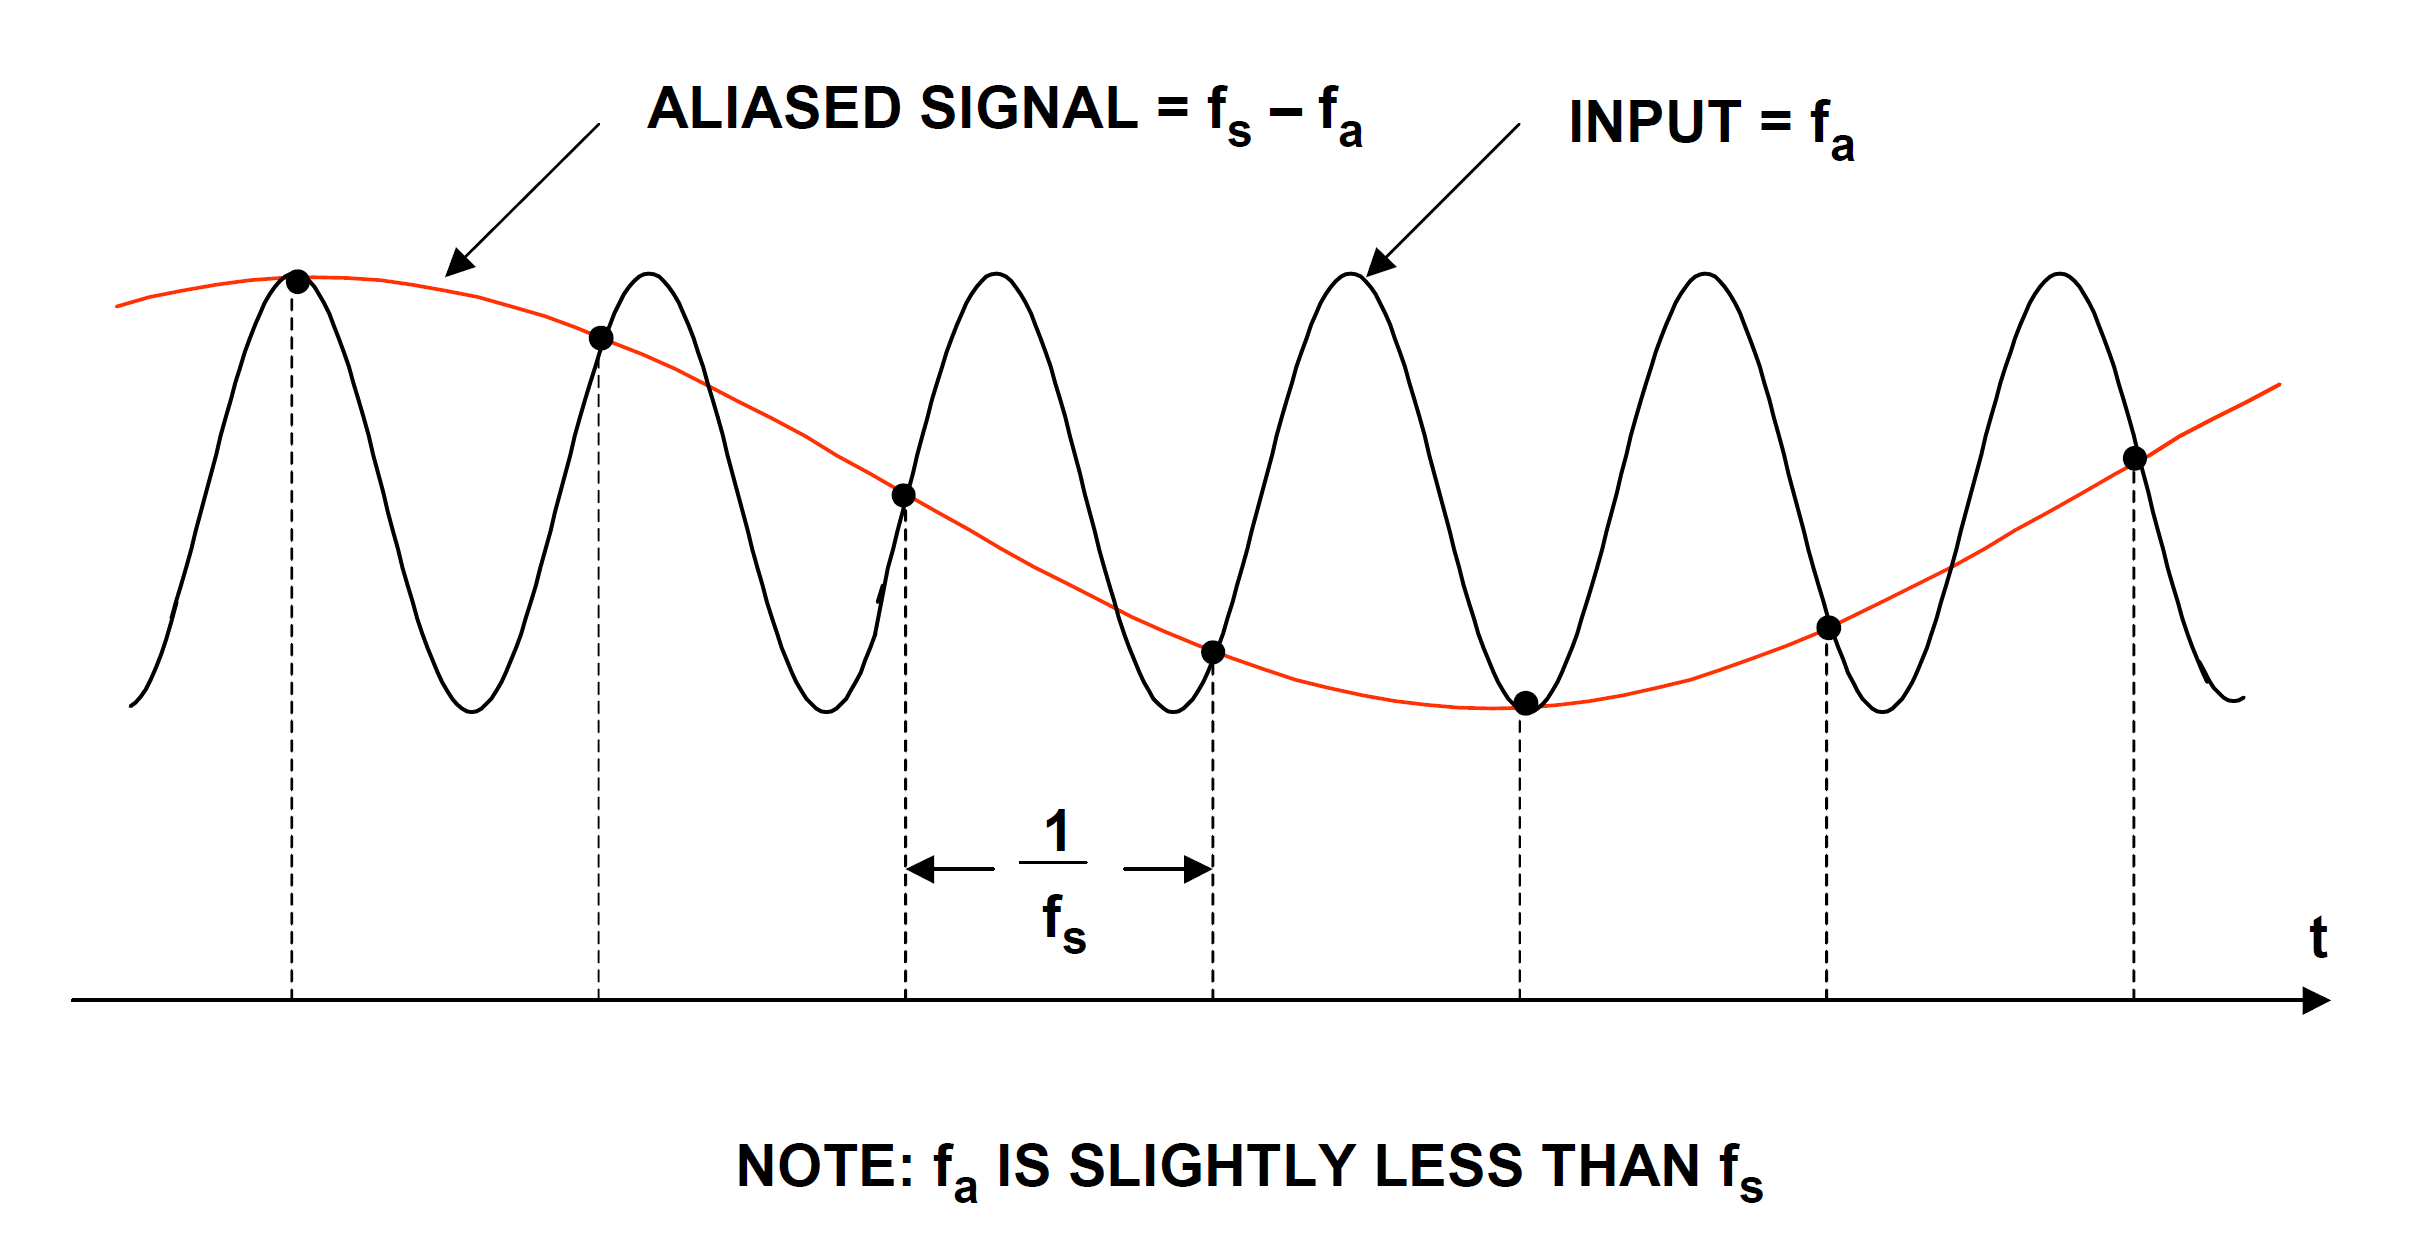
\includegraphics[width=\linewidth]{chap/02-theory/img/alias_t}  
		\caption{Aliasing in time domain}
		\label{fig:alias_t}
	\end{subfigure}
	\caption[Aliasing]{Analog signal with frequency $f_a$ sampled at $f_s$ respecting (A) and not respecting (B) the Nyquist criteria. \autoref{fig:alias_t} shows the effect of case B in time domain. \cite{walt}}
\end{figure}

%todo explain nyquist-bandwidth
%todo low-pass filter to get B/2<f_s? maybe


\paragraph{Sample-And-Hold-Amplifier}
\Glspl{adc} need a certain amount of time to sample the input signal.
If the level of the analog signal changes by more than one \gls{lsb} during this period, this can result in large errors in the output signal.
Therefore, so called \gls{sha} are used in front of the \gls{adc} to hold the input level constant for the needed amount of time.
The \gls{adc} sampling time needs to be timed in such way, that the analog-to-digital conversion falls into the hold period of the \gls{sha} and does not exceed into the sample period, for example like shown schematically in the diagram below. Thus, the upper frequency limitation is not determined by the \gls{adc} itself, but rather by the aperture jitter, bandwidth, distortion, etc. of the \gls{sha}. \cite{walt}



\begin{figure} [H]
	\centering
	\tikzexternaldisable
	\begin{tikztimingtable}
		[%
		timing/dslope=0.1,
		timing/name/.style={font=\sffamily\normalsize},
		timing/d/text/.style={font=\sffamily\normalsize},
		grayz/.style={timing/z/.append style={gray}},
		timing/n/.style={rectangle},
		timing/metachar={{K}[2]{#1l !{++(0,+.5\yunit)} N[rectangle,scale=.6]{\shortstack{#2}} !{++(0,-.5\yunit)} #1l}},
		timing/metachar={{J}[2]{#1h !{++(0,-.5\yunit)} N[rectangle,scale=.6]{\shortstack{#2}} !{++(0,+.5\yunit)} #1h}},
		]
		SHA & 1H 8K{HOLD} 8J{SAMPLE} 8K{HOLD} 3H\\
		Sampling & 5S A 15S A                    \\
	\end{tikztimingtable}
	\tikzexternalenable
\end{figure}
%todo why not save this as .tikz file and include it as a normal figure with caption?

In addition to the \gls{sha}, there is also the \gls{tha}.
Instead of a sample period, the \gls{tha} has a track period, where the output of the amplifier tracks the input signal (see also \autoref{fig:tha}).
When switching to hold mode, the signal at this instant is held. This is opposed to the \gls{sha}, where the output during sample mode is actually not defined and is set to the value of the input signal, only when switching into hold mode.
%todo explanation a bit confusing. use another timing diagram?

\begin{figure}[tbh]
	\centering
	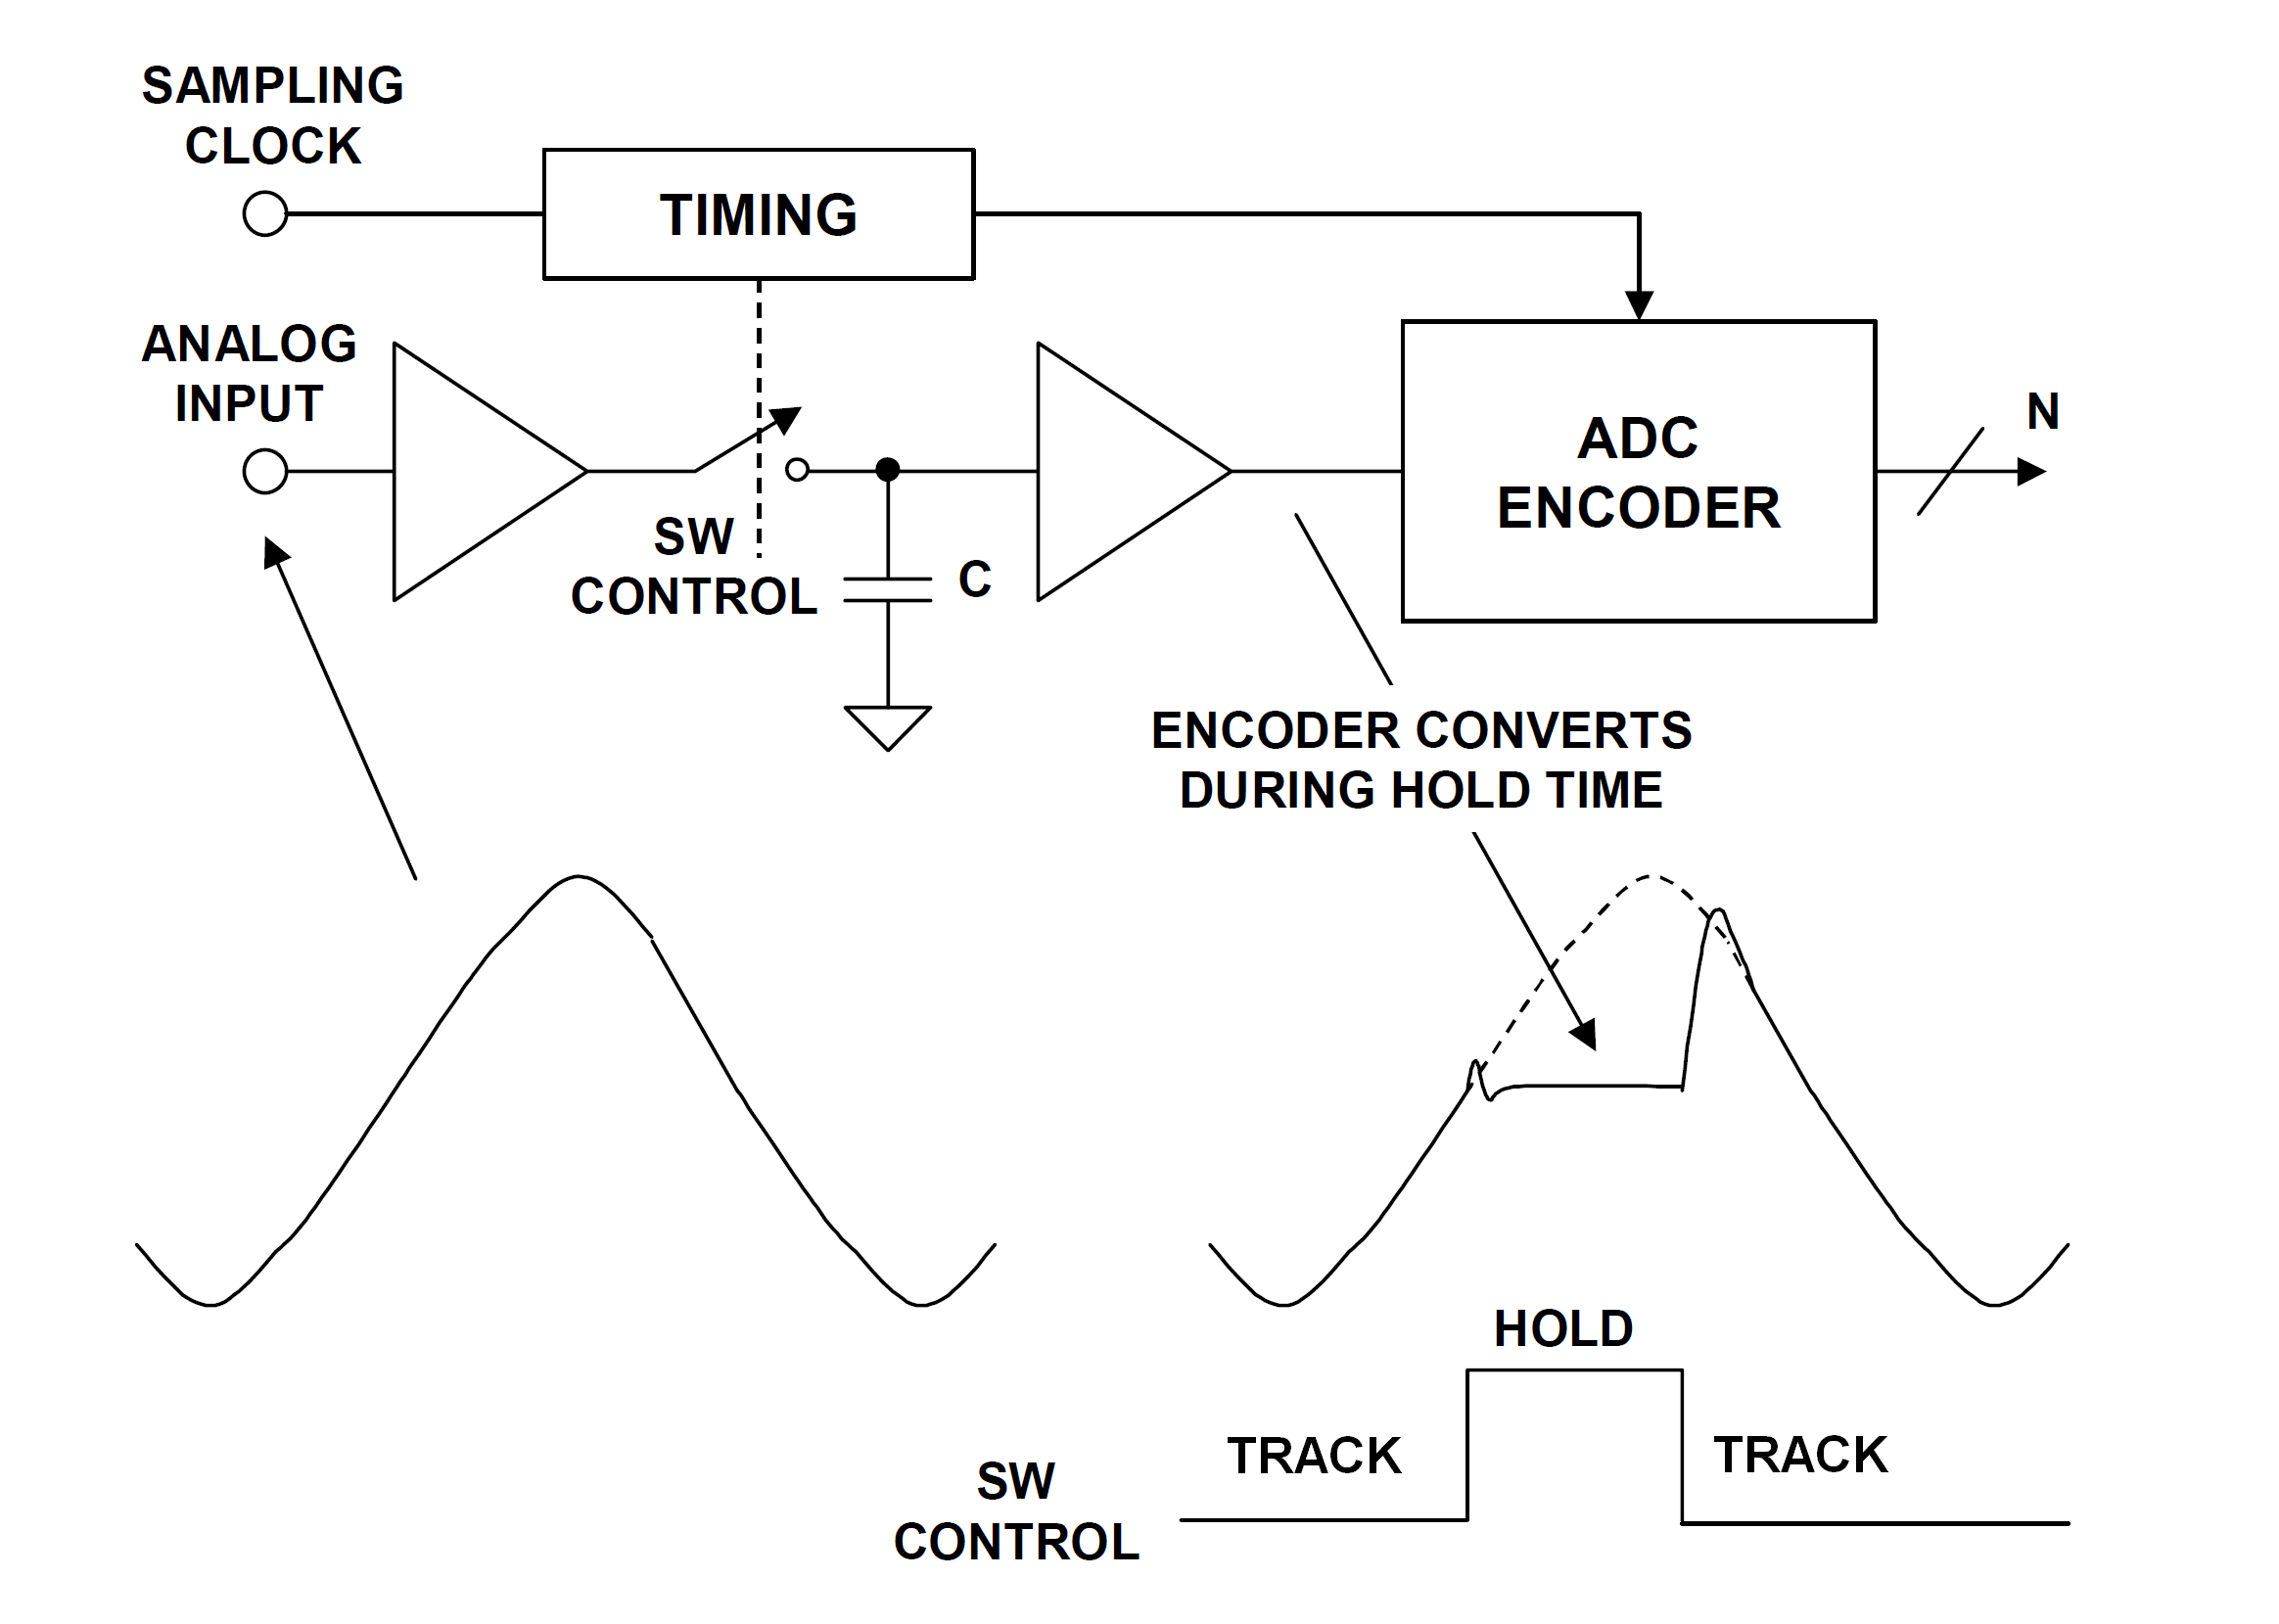
\includegraphics[width = \textwidth]{chap/02-theory/img/tha}
	\caption{Track-And-Hold-Amplifier schematic and principle \cite{walt}}
	\label{fig:tha}
\end{figure}

\subsubsection*{Characteristics of Analog-To-Digital-Converters}
For an ideal converter, the number of bits would be sufficient to fully characterize it.
Real \glspl{adc} however differ from the ideal behavior by introducing static and dynamic imperfections.
Different applications have different requirements, which leads to a number of specifications. These can be divided into the following categories \cite{Lundberg}:
\begin{itemize}[noitemsep]
	\item Quantization Noise
	\item Static parameters
	\item Frequency-domain dynamic parameters
	\item Time-domain dynamic parameters
\end{itemize}
This section provides an overview of these figures of merit. Which of these are needed to specify the necessary performance of the \gls{adc} has to be chosen for each application accordingly.

\paragraph{Quantization Noise}\label{par:quant_noise}
Even in an ideal N-bit converter there will be errors during the quantization, which behave like noise. The reason is that each N-bit word represents a certain range of analog input values, which is 1 \gls{lsb} wide and centered around a code center (see \autoref{fig:idealADC}) \cite{Lundberg}. The input voltage is assigned to the word of the nearest code center. This means that there will always be a difference between the corresponding voltage of the respective digital code $x_q(t)$ and the actual analog input voltage  $x(t)$. This difference is called the \textit{quantization error}. For an equidistant quantization with code width $q$ it is

\begin{equation}
\left| e_q(t) \right| = \left| x(t) - x_q(t) \right| \leq \frac{q}{2}.
\end{equation}
 \cite{puente2015} 

Assuming the error voltage uncorrelated and uniformly distributed, the theoretical (maximum) \gls{snr} of this \textit{quantization noise} can be calculated. In the time domain, the quantization error $e(t)$ can be approximated with a sawtooth signal:
\begin{equation}
e(t) = st, \quad -\frac{q}{2s} < t < \frac{q}{2s} 
\end{equation}
\begin{figure}[tbh]
	\centering
	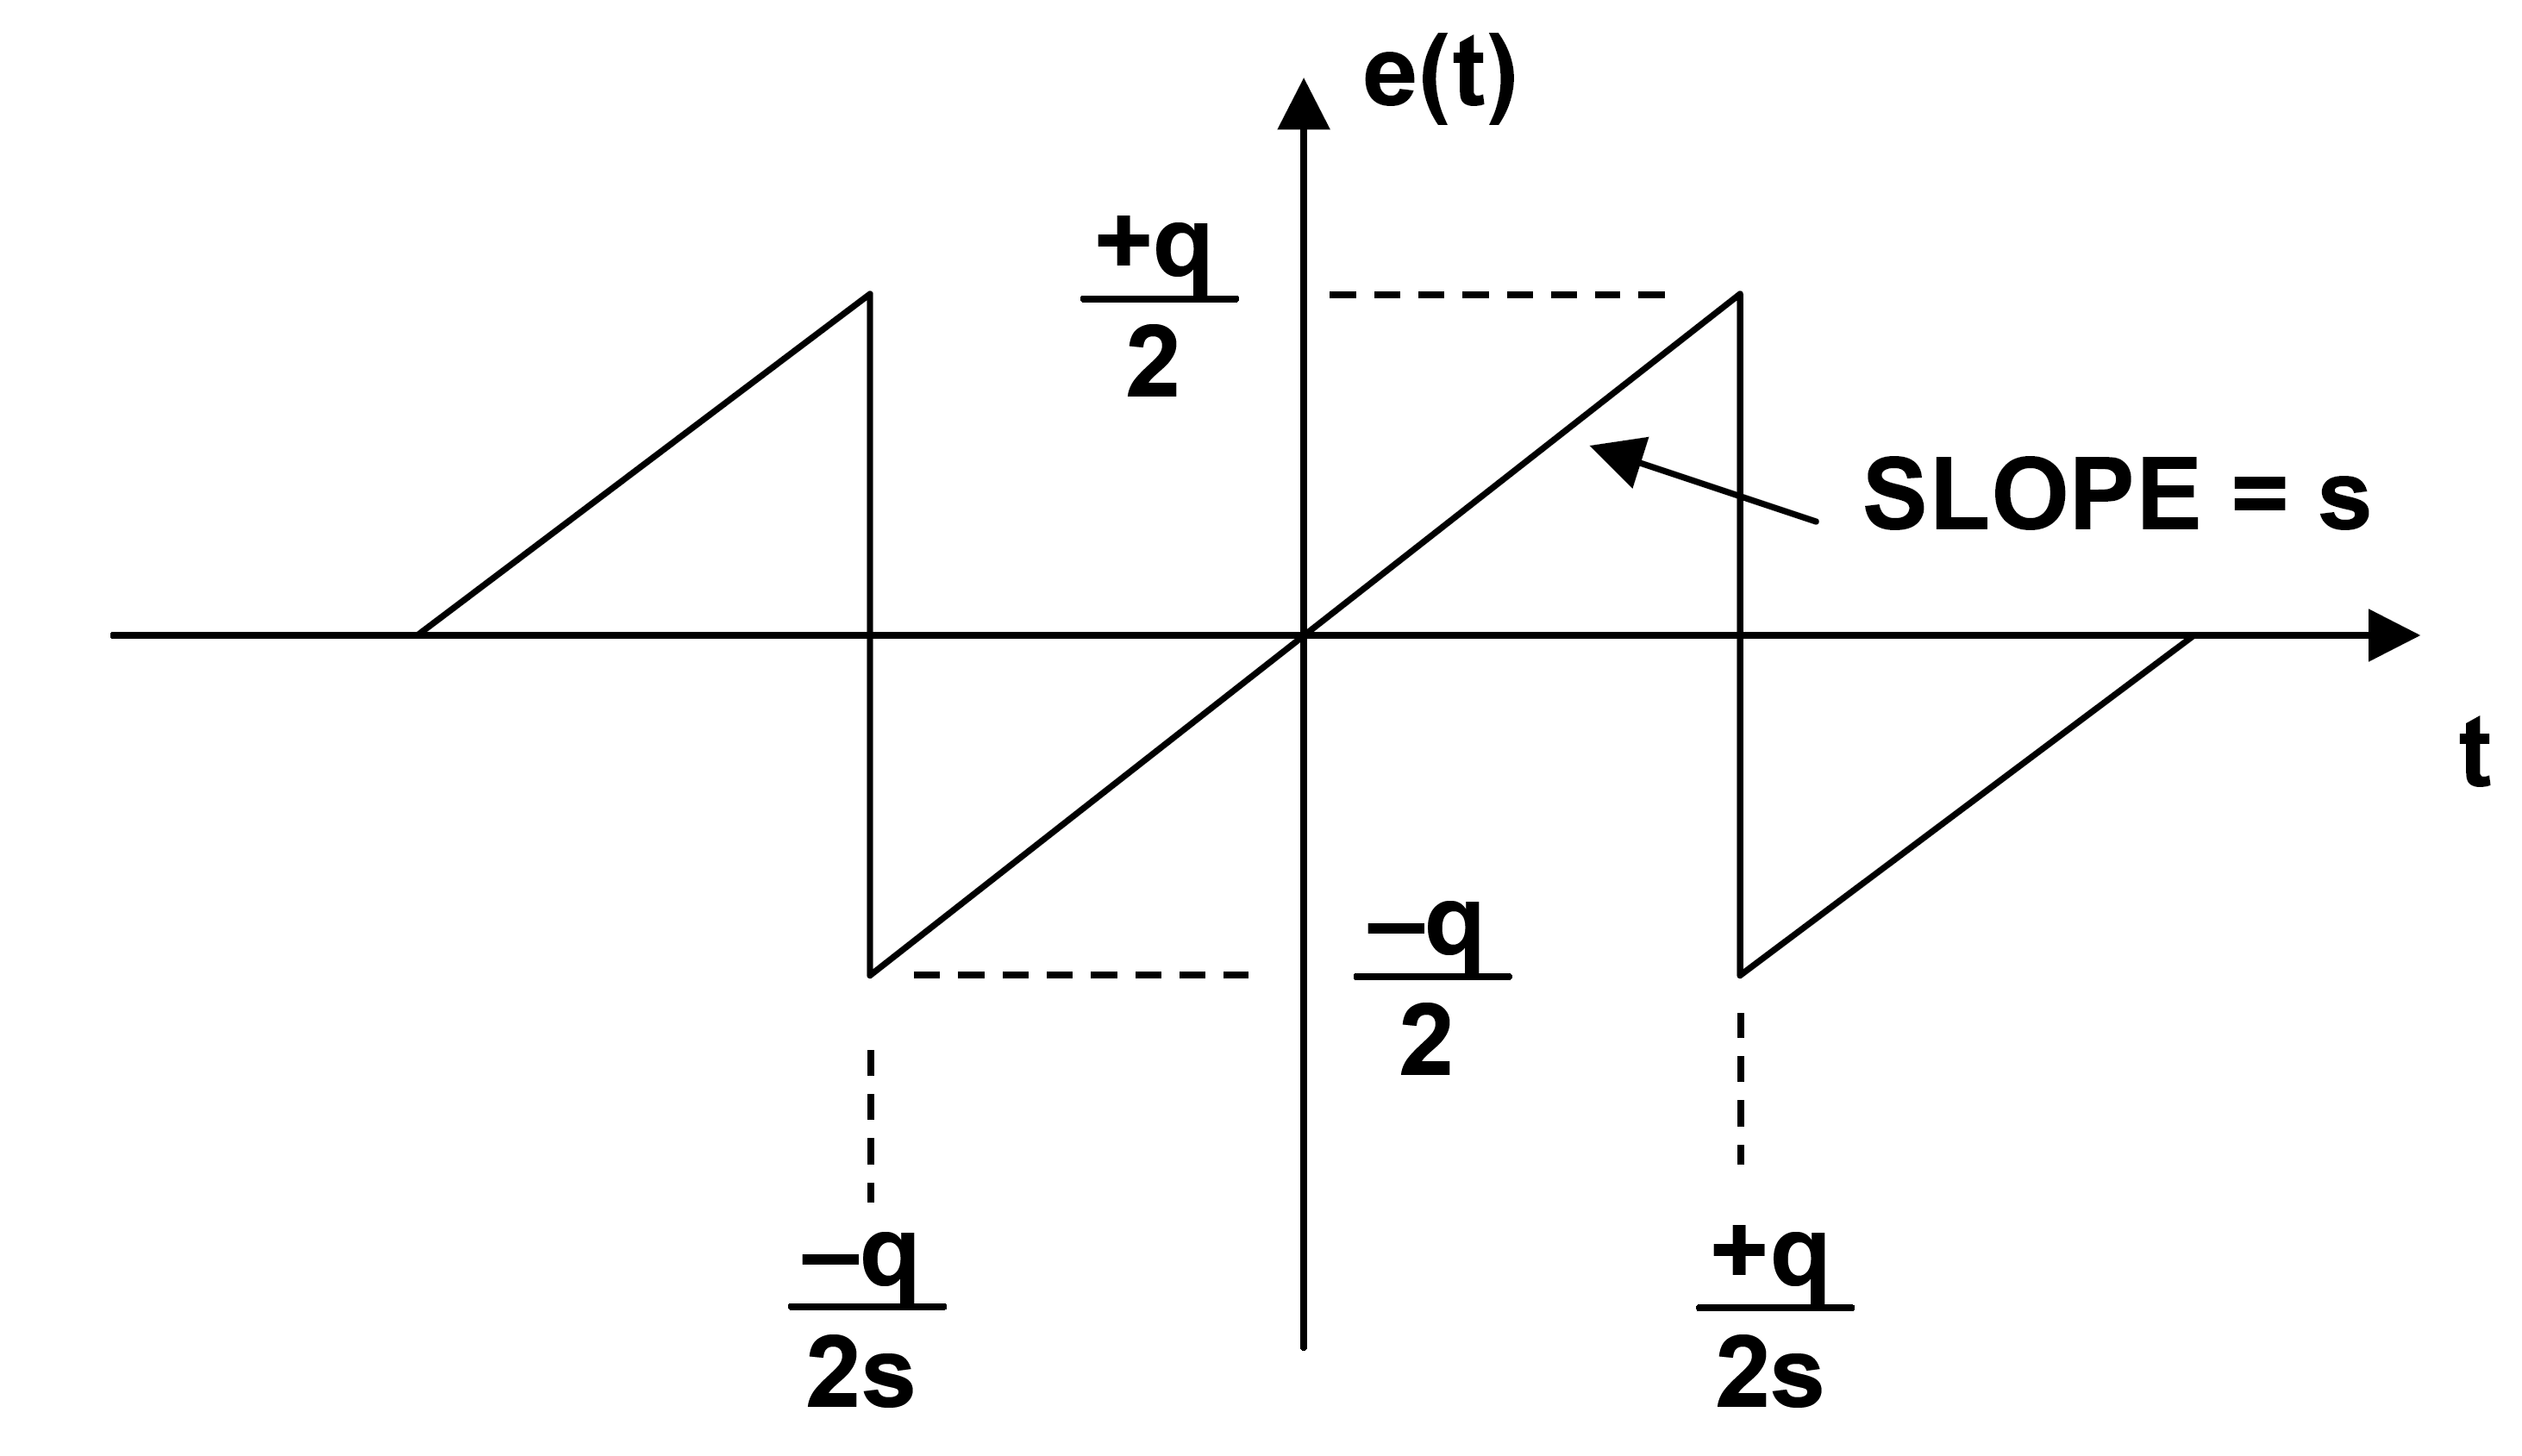
\includegraphics[width = 0.7\textwidth]{chap/02-theory/img/quantization_error.tikz}
	\caption{Quantization noise as function of time (redrawn from \cite{walt})}
	\label{fig:eq}
\end{figure}

The power of the quantization noise, which is assumed to be uncorrelated and broadband, can be calculated as the mean-square $e_{\text{rms}}^2$of $e(t)$ \cite{walt}:
\begin{equation}
P_{QN} = e_{\text{rms}}^{2} = \overline{e^{2}(t)} = \frac{s}{q}\int_{-q/2s}^{+q/2s} (st)^{2} dt = \frac{s^3}{q} \left[ \frac{t^3}{3}\right]_{-\frac{q}{2s}}^{+\frac{q}{2s}} = \frac{q^2}{12}
\end{equation}

To calculate the maximal \gls{snr} of an ideal converter, a full-scale input sine wave is assumed:
\begin{equation}
u(t) = u_s \sin(2\pi f t) = \frac{2^{N}q}{2}\sin(2\pi f t)  = 2^{N-1}q \sin(2\pi f t)
\end{equation}
With the effective value of the signal amplitude
\begin{equation}
u_{\text{eff}} = \frac{u_s}{\sqrt{2}} = \frac{2^{N-1}q}{\sqrt{2}}
\end{equation}
\gls{snr}
\begin{equation}
\text{SNR} = \frac{P_{\text{signal}}}{P_{\text{noise}}} = \frac{u_{\text{eff}}^{2}}{e_{\text{rms}}^{2}} = \frac{2^{2N-2}q^2/2}{q^2/12} = 2^{2N} \cdot 1.5.
\end{equation}
In decibel:
\begin{equation}\label{eq:idealSNR}
\text{SNR}|_{\text{dB}} = 10\log\left(2^{2N}\cdot 1.5\right) = 6.02 N + 1.76
\end{equation}
\cite{puente2015} \cite{walt}



\paragraph{Static parameters}
\textit{Static parameters} are specifications, which can be measured at low speed/DC. 
\paragraph{Accuracy}
\textit{Accuracy} is the total error with which an \gls{adc} can convert a known voltage, which includes the effects of:
\begin{itemize}[noitemsep]
	\item Quantization error
	\item Gain error
	\item Offset error
	\item Nonlinearities
\end{itemize}
\cite{Lundberg}
\paragraph{Resolution}
\textit{Resolution} is the number of bits $N$ of the \gls{adc}. Depending from the resolution are the size of the \gls{lsb}, which in its turn determines the dynamic range, code widths and quantization error.
\paragraph{Dynamic Range}
The \textit{dynamic range} represents the ratio between smallest possible output (\gls{lsb} voltage) and the largest possible output (full-scale voltage). It can be calculated as
\begin{equation}
	20 \log 2^{N} \approx 6N.
\end{equation}
\paragraph{Offset and Gain Error}
The \textit{offset error} is the deviation of the first transition voltage from the ideal $1/2$ \gls{lsb}. \textit{Gain Error} defines the deviation of the slope of the line going through the zero and full-scale point of the transfer function. These errors can easily be corrected by calibration. \autoref{fig:offsetErr} visualizes the effects of both offset and gain error. 
\begin{figure}[tbh]
	\centering
	\includegraphics[width = 0.7\textwidth]{chap/02-theory/img/offset_err.tikz}
	\caption[Effects of Offset and Fain error in ADC]{Offset and Gain Error in the \gls{adc} characteristic transfer function. Notice the difference between the line going through the code centers (dashed) and the line of an ideal \gls{adc} (dotted)}
	\label{fig:offsetErr}
\end{figure}


\paragraph{Integral and Differential Nonlinearity Distortion} 
\textit{\gls{inl}} in the transfer function is the distance of the code centers from the ideal line. It results from the integral nonlinearities of the front-end, \gls{sha} and also the \gls{adc} itself. \cite{walt} These nonlinearities depend on the input signal amplitude. \cite{Lundberg}
%todo not sure about the \textit + \gls

\textit{\gls{dnl}} is the deviation in code width from the ideal width of 1 \gls{lsb}. This nonlinearity stems exclusively from the encoding process in the \gls{adc}. \cite{walt} It not only depends on the input signal amplitude, but also on the positioning along the transfer function. \cite{Lundberg}

\begin{figure}[tbh]
	\centering
	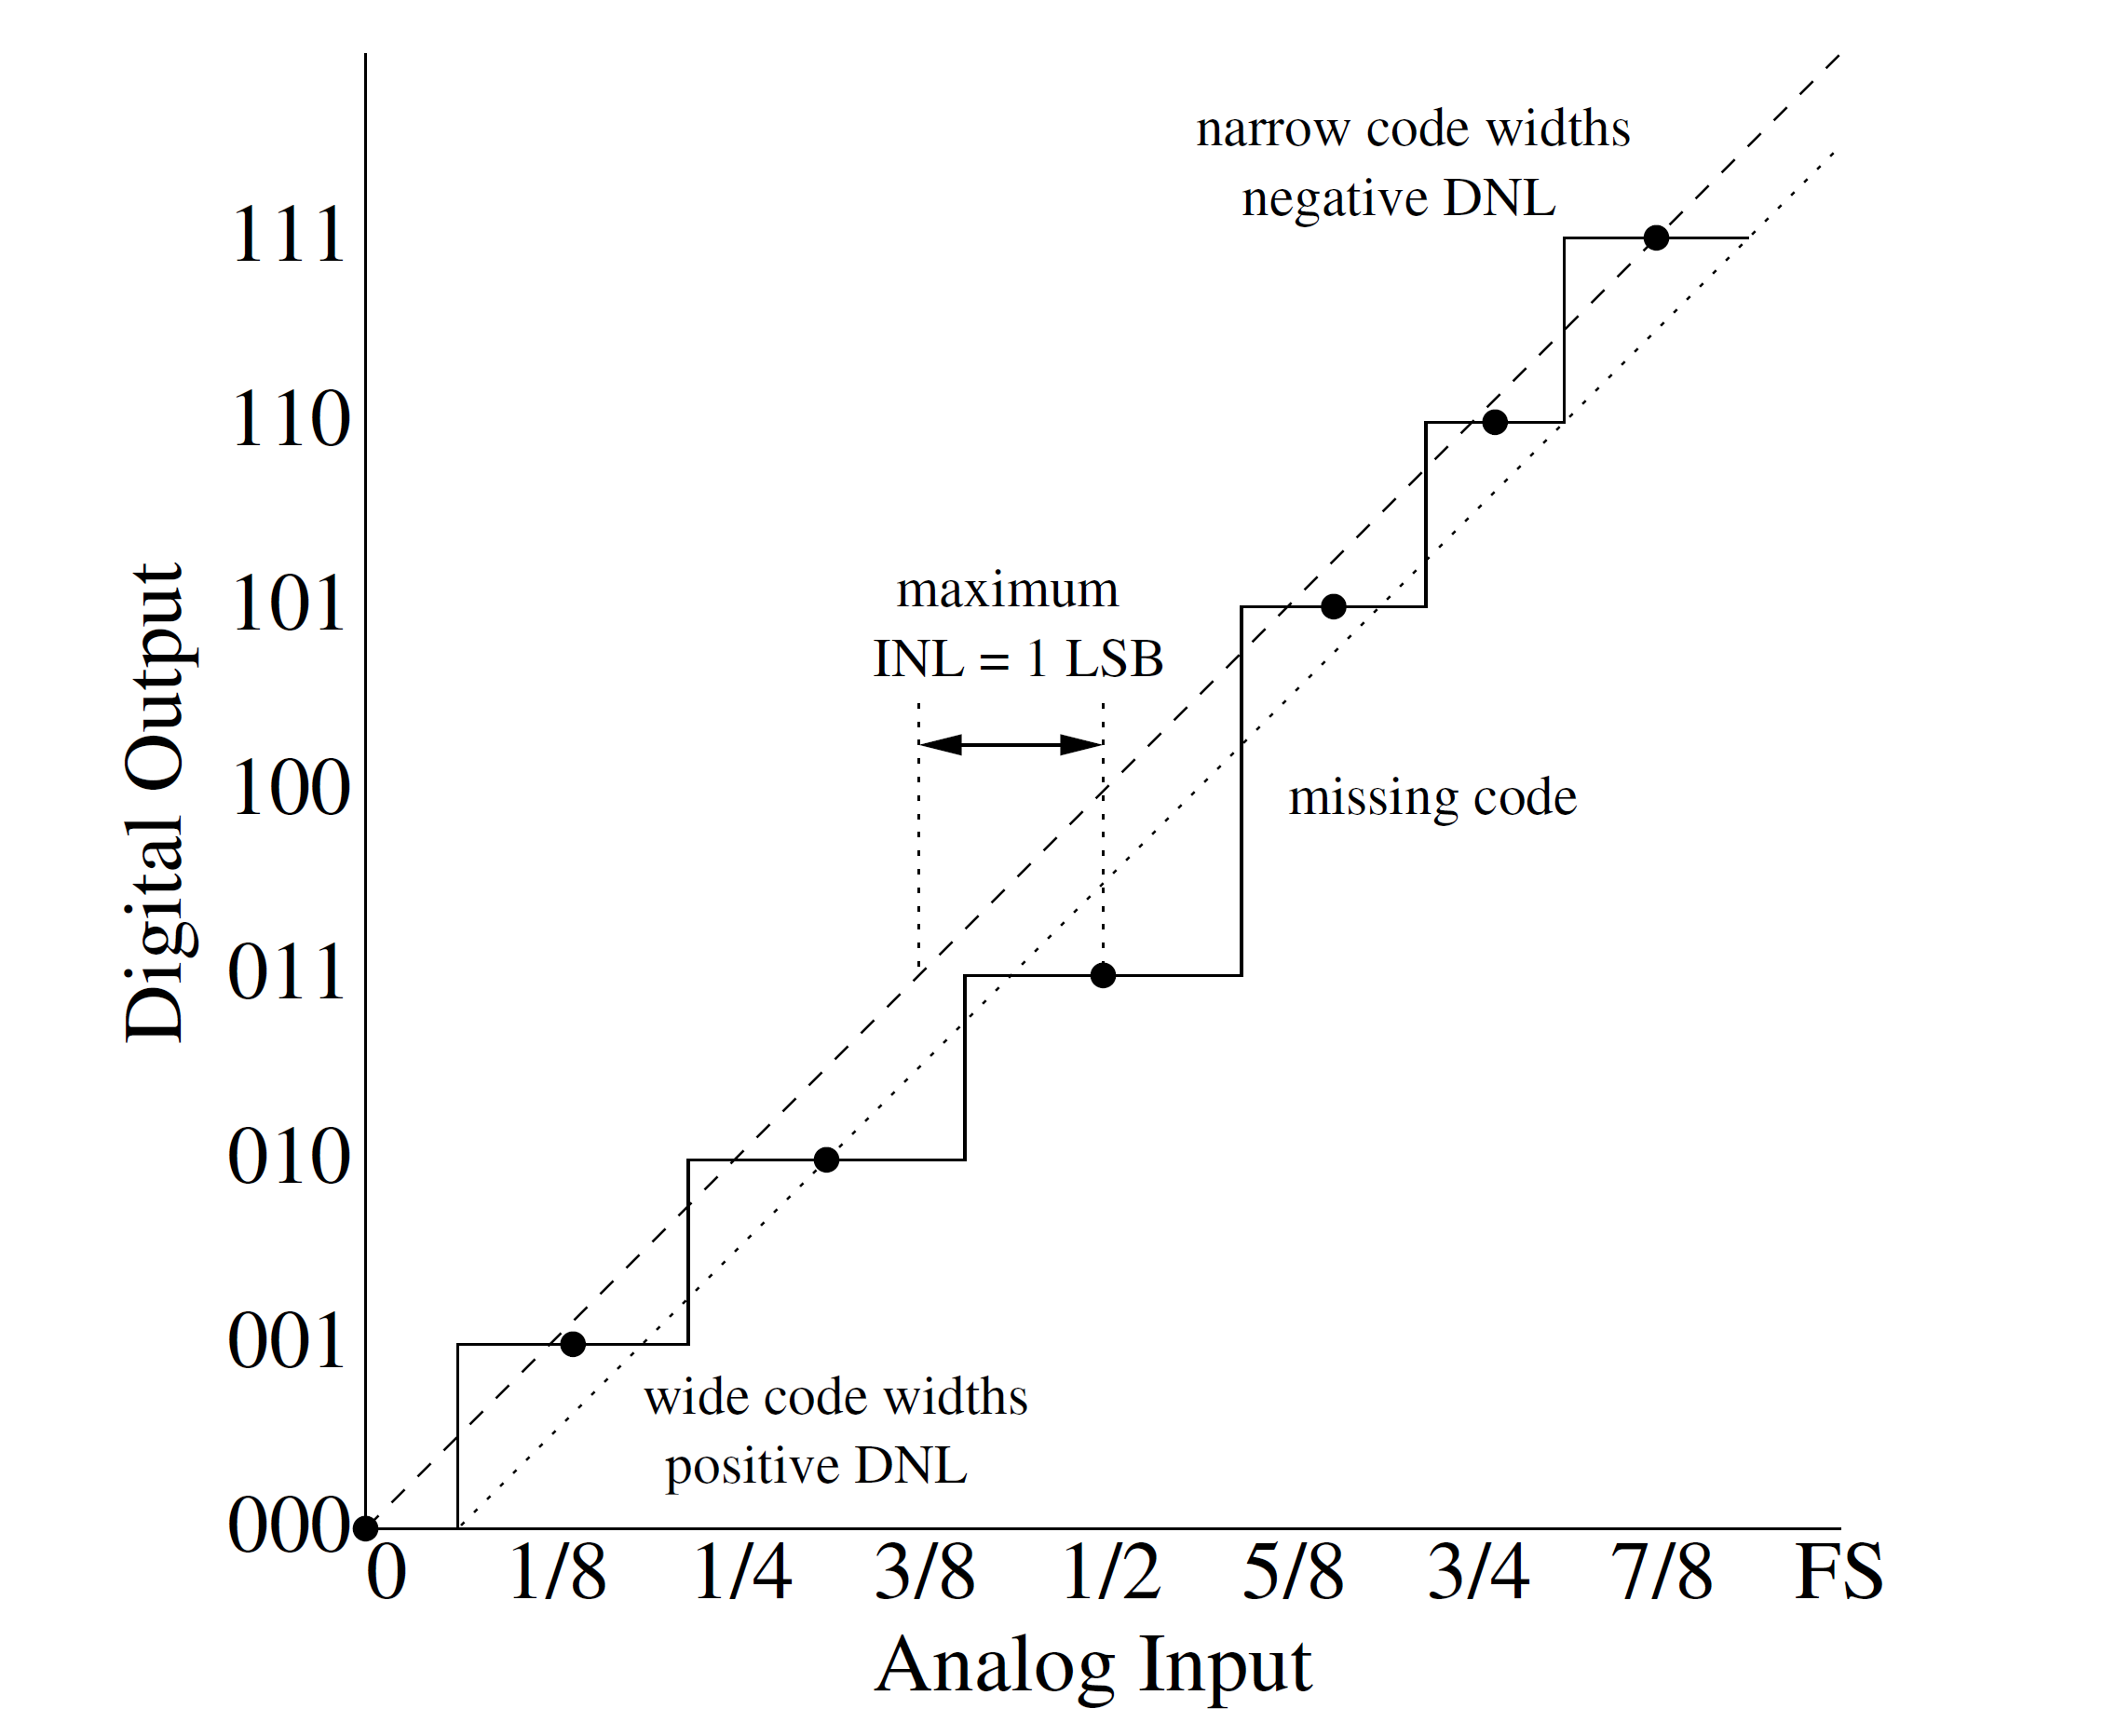
\includegraphics[width = 0.7\textwidth]{chap/02-theory/img/dnld}
	\caption{Placeholder: Integral and Differential Nonlinearity Distortion \cite{Lundberg}}
	\label{fig:nld}
\end{figure}
%todo to tikz

\paragraph{Frequency-Domain Dynamic Parameters}
Real \glspl{adc} have additional noise sources and distortion processes. \textit{Noise} relates to any unwanted (random or deterministic) signal, which interferes with the desired signal (e.g. additive or quantization noise). \textit{Distortion} is the term for the change of the original signal. These have an impact on the \gls{adc} behavior. 

In an \glspl{adc} (with built-in \gls{sha}) there are a couple of sources, which introduce noise and distortion:
\begin{itemize}
	\item \textbf{Input Stage:} Wideband noise, nonlinearity and bandwidth limitation
	\item \textbf{\gls{sha}:} Nonlinearity, aperture jitter(see paragraph about Time-Domain Dynamic Performances)  and bandwidth limitation
	\item \textbf{\gls{adc}:} Quantization noise, nonlinearity
\end{itemize}

In the following, an overview of the metrics for quantification of these imperfections is given. 


\paragraph{Signal-to-Noise-and-Distortion Ratio}
\textit{\gls{sinad}} (also called SNDR or S/N+D) denotes the ratio between the \gls{rms} of the signal amplitude to the mean value of the Root-Sum-Square (RSS) of all other spectral components, including harmonics, but excluding  DC (\SI{0}{\hertz}). \gls{sinad} is a good indication over the general dynamic performance of the \gls{adc}, as it includes all contributions from noise and distortion.

\paragraph{Effective-Number-Of-Bits}
The \textit{\gls{enob}} expresses the \gls{sinad} in terms of bits. It can be calculated as
\begin{equation}
	\text{ENOB} = \frac{\text{SINAD}-\SI{1.76}{\decibel}}{\SI{6.02}{\decibel}/\text{bit}}. \quad \cite{walt2009}
\end{equation}
This is derived from solving the equation of the "ideal \gls{snr}" \autoref{eq:idealSNR} for the number of bits $N$ and substituting \gls{snr} with \gls{sinad}. This however means, that this parameter assumes a full-scale input signal. Expressing the \gls{enob} for a smaller signal amplitude requires measuring the \gls{sinad} at this level and a correction factor. \cite{walt}


\paragraph{Spurious-Free Dynamic Range}
\textit{\gls{sfdr}} indicates the dynamic range of the converter, which can be used, before there is interference or distortion from spurious components with the fundamental signal. \cite{Lundberg} The \gls{sfdr} is calculated as the \gls{rms} value of the fundamental signal to the \gls{rms} value of the worst spurious signal, i.e. the highest spur in the spectrum. It is measured over the whole Nyquist-Bandwidth (DC (\SI{0}{\hertz}) to $f_s/2$, $f_s$ being the \gls{adc} sampling rate). The spur may or may not be a harmonic of the fundamental signal. \cite{walt2009} \cite{Lundberg}

The \gls{sfdr} is an important characteristic in the sense, that it indicates the smallest signal which can still be distinguished from a strong interfering signal. \cite{walt2009} 

\autoref{fig:sfdr} illustrates the \gls{sfdr} in terms of \gls{dbfs} and \gls{dbc}.

\begin{figure}[tbh]
	\centering
	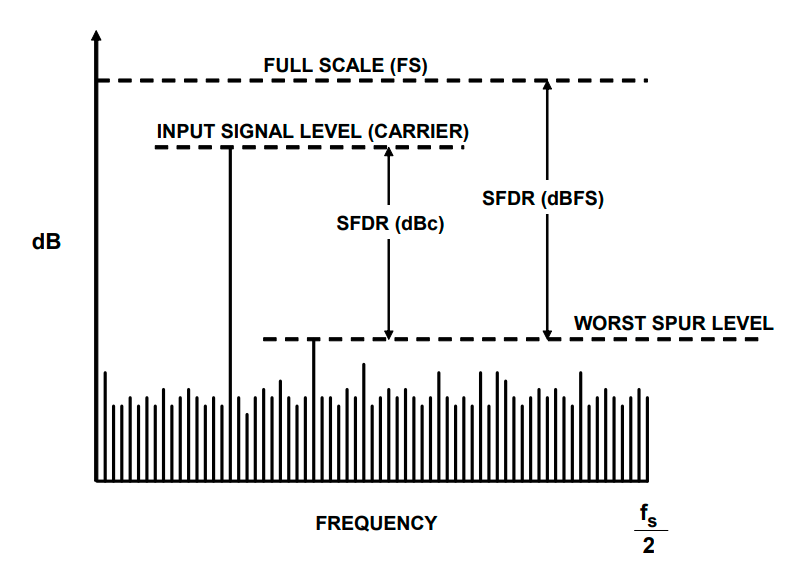
\includegraphics[width = \textwidth]{chap/02-theory/img/sfdr}
	\caption{Placeholder: SFDR \cite{walt2009}}
	\label{fig:sfdr}
\end{figure}

\paragraph{Total Harmonic Distortion}
The \textit{Total Harmonic Distortion} describes the ratio of the \gls{rms} sum of the first five harmonic components (or aliased versions of them) to the \gls{rms} of the considered fundamental signal.  \cite{Lundberg}

\paragraph{Effective Resolution Bandwidth}
\textit{Effective Resolution Bandwidth} denotes the frequency of the input signal, at which the \gls{sinad} has fallen by \SI{3}{\decibel} ($\eqdev$ 0.5 bit in terms of \gls{enob}) compared to the \gls{sinad} at lower frequency range. \cite{Lundberg}

\paragraph{Analog Input Bandwidth}
\textit{Analog Input Bandwidth} is the analog input frequency at which the power of the fundamental is reduced by 3dB with respect to the low-frequency value.

\paragraph{Full-Linear Bandwidth}
The \textit{Full-Linear Bandwidth} is defined as the frequency at which the slew-rate (SR) of the \gls{sha} starts to distort the input signal by a specified value. \cite{Lundberg} The slew-rate is defined as the rate of how much the voltage $v$ changes against time $t$:
\begin{equation}
	\text{SR} = \frac{dv}{dt}
\end{equation}
A SR of \SI{1}{\volt \per \micro \second} for example means, that the output of the amplifier can not change more than \SI{1}{\volt} over the course of \SI{1}{\micro \second}.\cite{2021Slew} 

\paragraph{Time-Domain Dynamic Parameters}
Time-Domain Dynamic parameters describe the deviation of the converter's behavior from the ideal one in time domain. 
\paragraph{Aperture Delay}
\textit{Aperture Delay} (or \textit{aperture time}) is defined as delay between the triggering of the converter (e.g. rising edge of the sampling clock) and the actual conversion of the input voltage into the digitized value. \cite{Lundberg}
\paragraph{Aperture Jitter}
\textit{Aperture jitter} describes the sample-to-sample variation in aperture delay. Jitter can cause significant error in the voltage and decreases the overall \gls{snr} of a converter. Especially for high-speed \glspl{adc} jitter poses a limit in performance.

Assuming a full-scale sinus-wave $V_{\text{in}}$ as input signal with 
\begin{equation}
	V_{\text{in}} = V_{\text{FS}} \sin (\omega t)
\end{equation}
the maximal slope of this signal is then
\begin{equation}
	\frac{dV_{\text{in}}}{dt}\Bigr|_{\text{max}} = \omega V_{\text{FS}}
\end{equation}
Aperture jitter $\Delta t_{\text{rms}}$ occuring during the sampling of this maximal slope produces the \gls{rms} voltage error 
\begin{equation}
	\Delta V_{\text{rms}} = \omega  V_{\text{FS}} \Delta t_{\text{rms}} = 2 \pi f  V_{\text{FS}} \Delta t_{\text{rms}}.
\end{equation}
As variations in aperture time occur randomly, these errors behave like a random noise source. This way, a \gls{sjnr} can be defined as
\begin{equation}
	\text{SJNR} = 20 \log \left( \frac{V_{\text{FS}}}{\Delta V_{\text{rms}}} \right) = 20 \log \left( \frac{1}{2 \pi f  V_{\text{FS}}} \right)
\end{equation}

The voltage error due to jitter and the \gls{sjnr} for different aperture jitter values are shown in \autoref{fig:ap_jit}.

\begin{figure}[tbh]
	\centering
	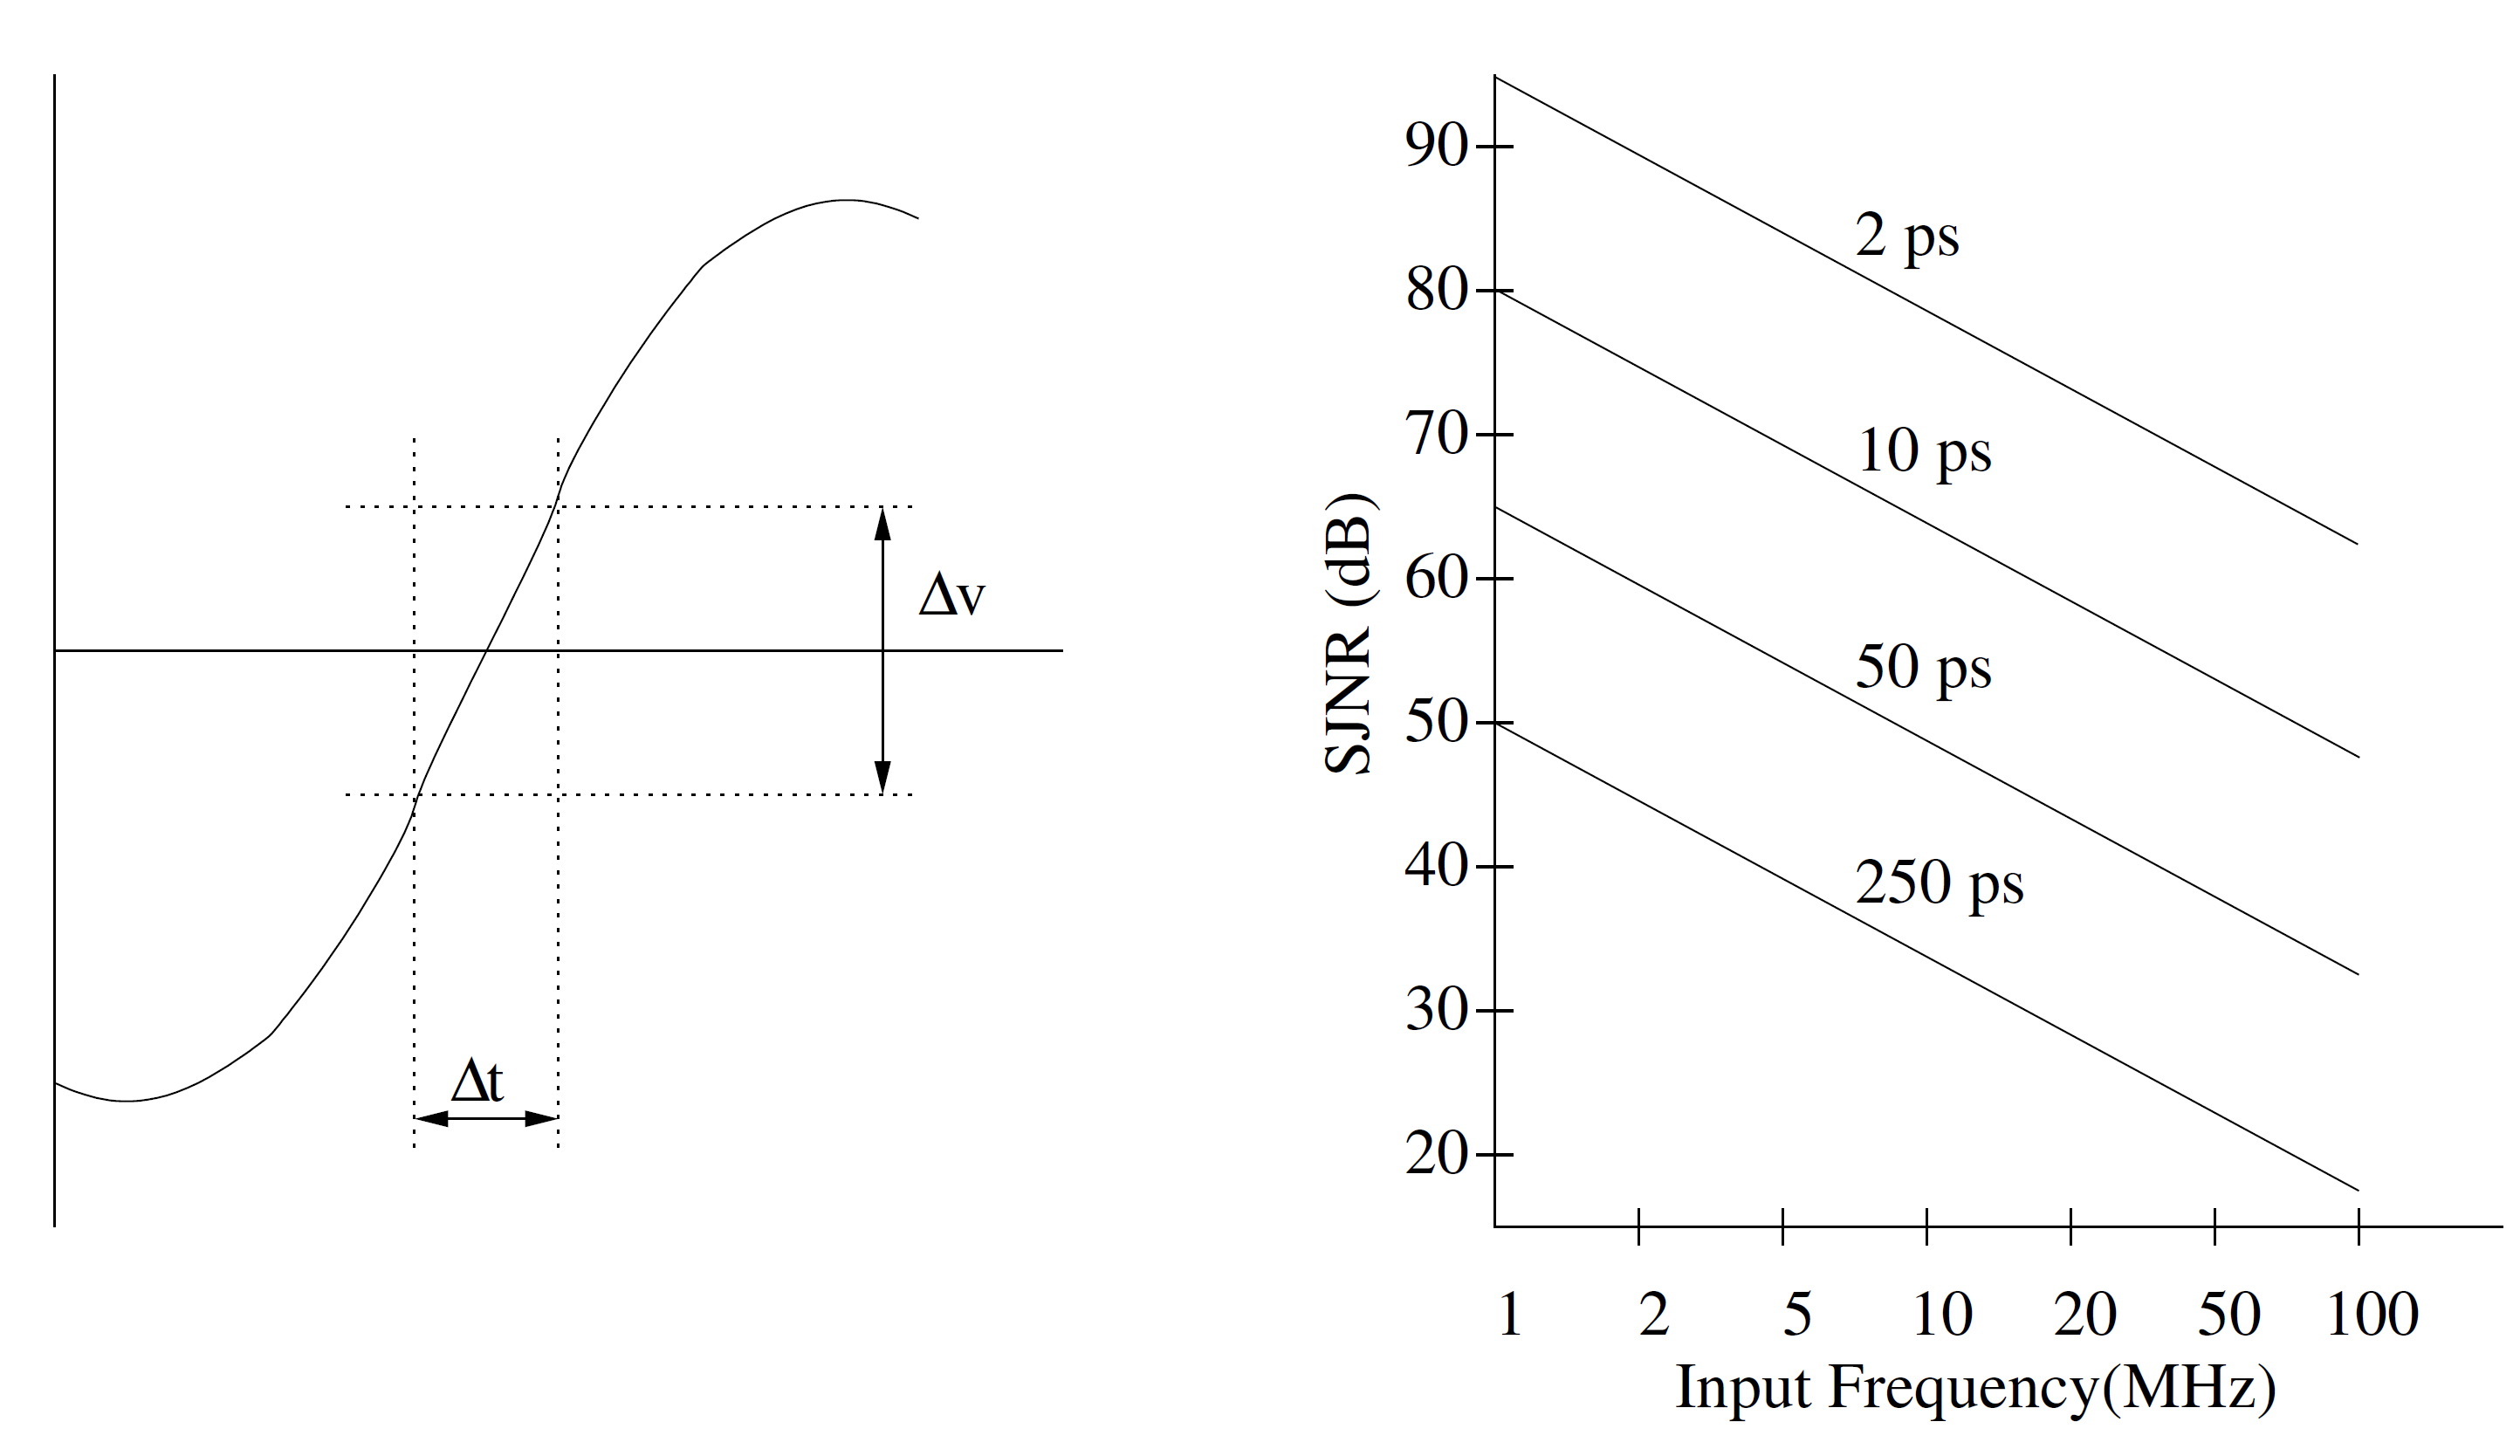
\includegraphics[width = \textwidth]{chap/02-theory/img/ap_jit}
	\caption{Placeholder: Effects of aperture jitter and SJNR \cite{Lundberg}}
	\label{fig:ap_jit}
\end{figure}
%todo to tikz

\paragraph{Transient Response}
The \textit{transient response} denotes the settling time of an \gls{adc} until full accuracy ($\pm$ 1/2 \gls{lsb})

\subsubsection*{Time Interleaving for Higher Sample Rates}
In the \textit{Time Interleaving} technique multiple \glspl{adc} are used in such way, that allows to sample data at a faster rate, than the respective sample rate of each individual \gls{adc}. The principle is based on time-multiplexing an array of $M$ identical \glspl{adc} (see \autoref{fig:adc_interleaving}), each sampling at $f_c = f_s/M$ individually. This means, the \glspl{adc} are clocked in such a way, that they start their respective conversion cycle shortly one after another. At time $t_0$ the first \gls{adc} starts converting the input signal $V_i(t_0)$, after a time delay $\Delta t_i$ the second starts converting the signal $V_i(t_0 + t_i)$, the third converts $V_i(t_0 + 2t_i)$ and so on. After the $M$-th \gls{adc} has sampled the signal $V_i(t_0 + (M-1)t_i)$, the whole cycle starts anew with the first converter. \cite{mangrob}

\begin{figure}[tbh]
	\centering
	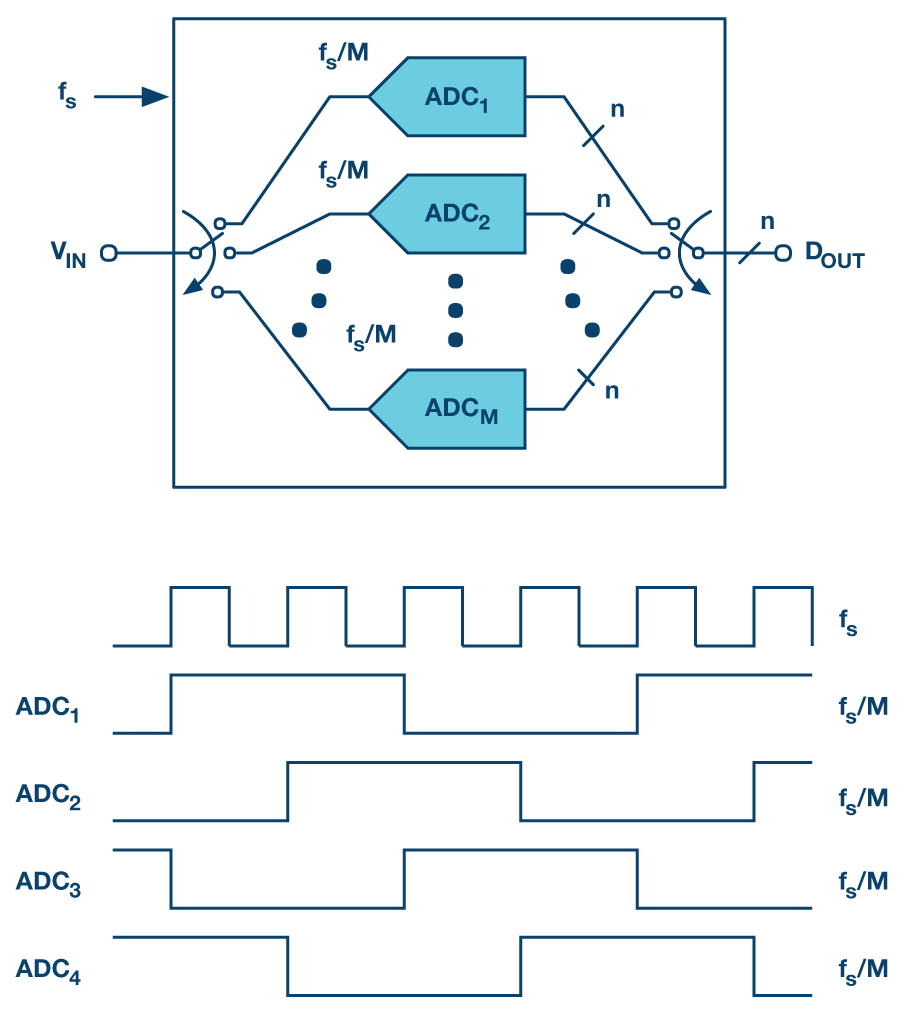
\includegraphics[width = \textwidth]{chap/02-theory/img/adc_inter}
	\caption[Time Interleaving]{Placeholder: An array of $M$ time interleaved $N$-bit \glspl{adc} with example of clocking scheme for the case of $M$ = 4 \cite{mangrob}}
	\label{fig:adc_interleaving}
\end{figure}
%todo to tikz

\paragraph{Challenges}
Spurs appear in the spectrum. There are several reasons for this.

First reason is the \textit{offset mismatch} between den \glspl{adc}. Each \gls{adc} has an DC offset value. Considering as example an interleaving structure with two \glspl{adc} and a constant input voltage: when the samples are acquired back and forth between the two \glspl{adc}, the resulting output will switch back and forth between two levels due to the different offset levels. This output switches at the frequency $f_s/2$ and therefore introduces an additional frequency component in the spectrum (see \autoref{fig:offset_mm}). The magnitude of the spur depends on the offset difference between the \glspl{adc}. \cite{Harris2019}

\begin{figure}[tbh]
	\centering
	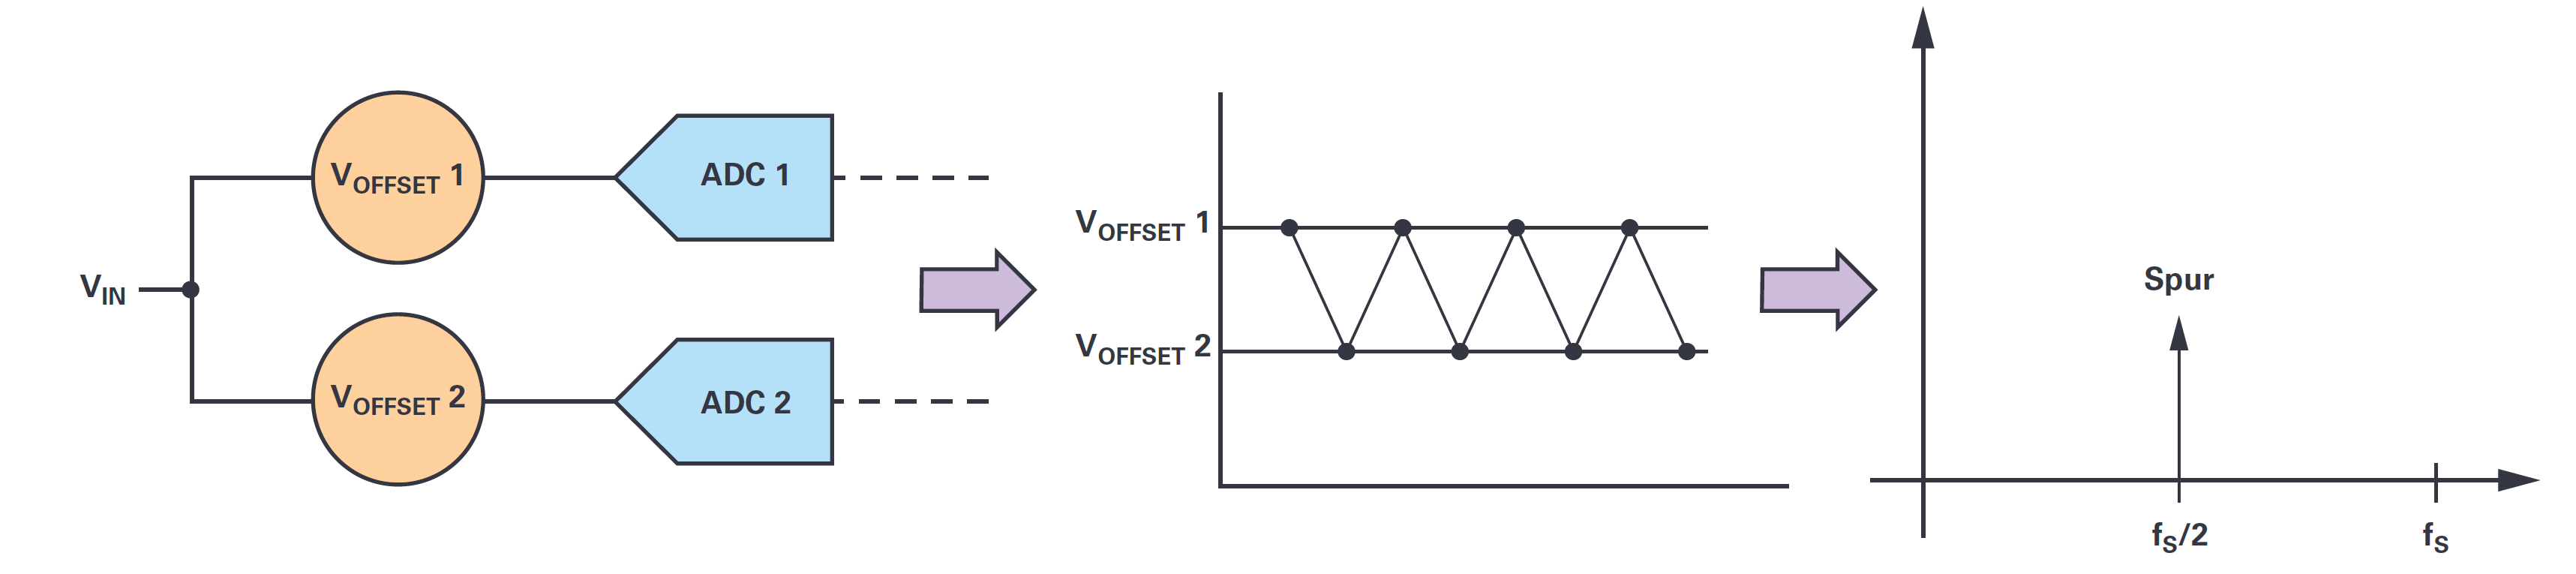
\includegraphics[width = \textwidth]{chap/02-theory/img/offset_mm}
	\caption{Placeholder: Offset-Mismatch in Interleaving \cite{Harris2019}}
	\label{fig:offset_mm}
\end{figure}

Besides of the offset also the gain of the converters can be mismatched. This \textit{gain mismatch} has a frequency component to it, which in case of an input signal of the frequency $f_{\text{in}}$ results in a spur at $f_s/2 \pm f_{\text{in}}$ (see \autoref{fig:gain_mm}). \cite{Harris2019}
\begin{figure}[tbh]
	\centering
	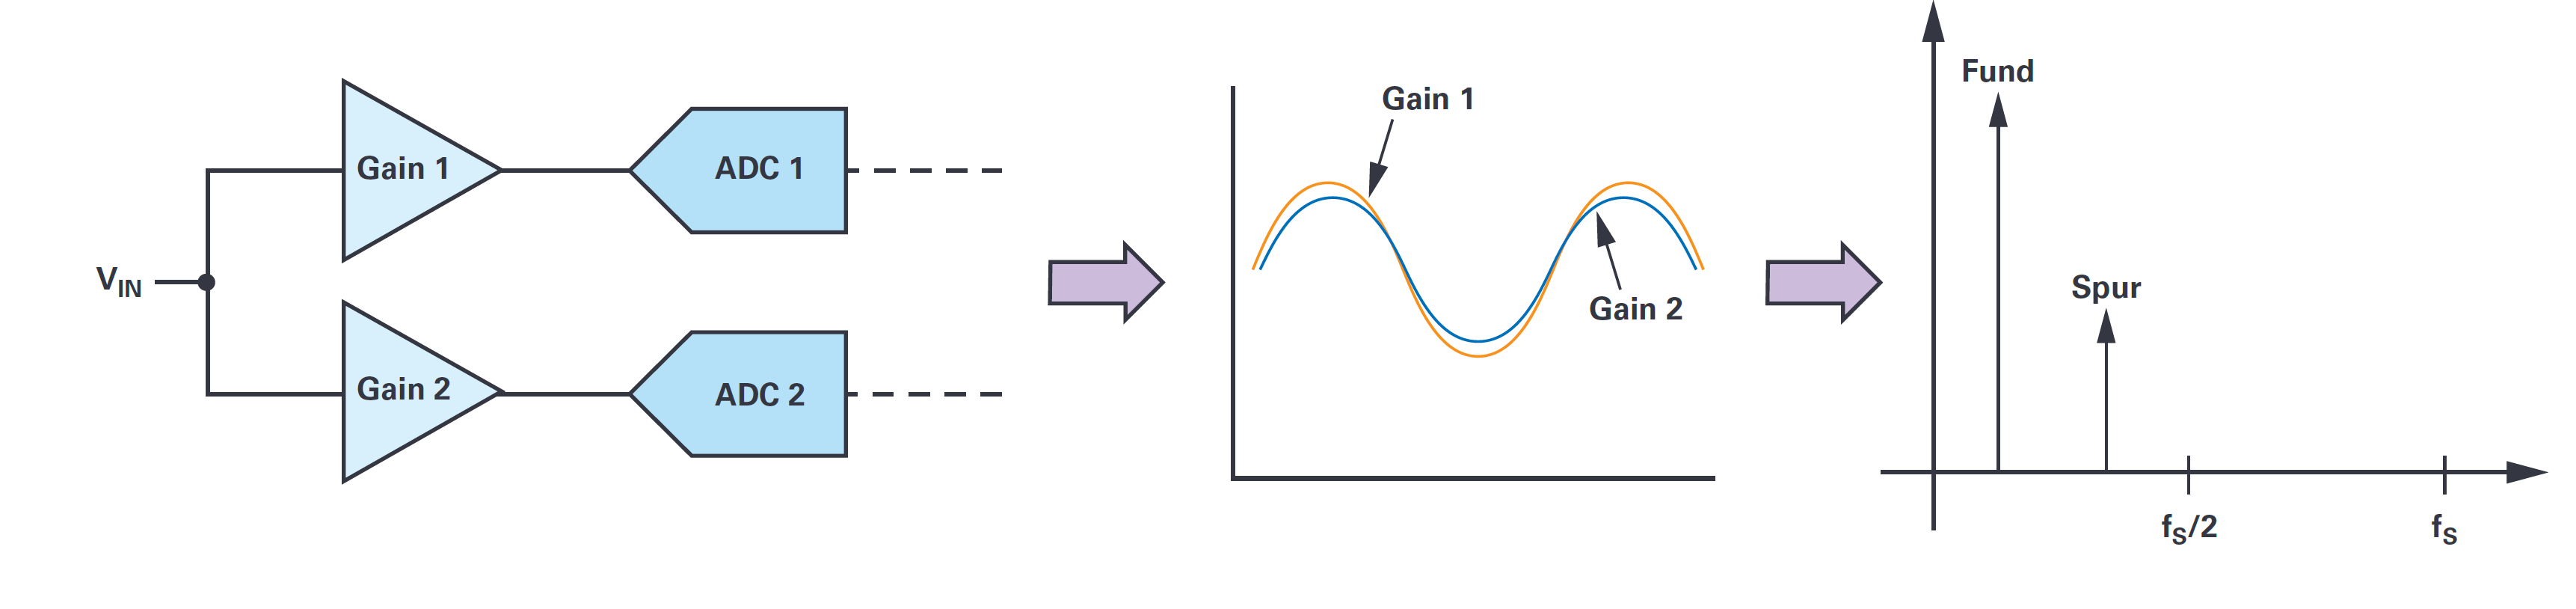
\includegraphics[width = \textwidth]{chap/02-theory/img/gain_mm}
	\caption{Placeholder: Gain-Mismatch in Interleaving \cite{Harris2019}}
	\label{fig:gain_mm}
\end{figure}

In the time domain, \textit{timing mismatch} due to group delay in the analog circuitry of the \gls{adc} and clock skew\footnote{Difference in arrival time of the clock signal at different components.} can occur. The group delay in analog circuitry can vary between the converters. Furthermore, the clock skew has on the one hand an aperture uncertainty component at each of the \glspl{adc} and on the other hand a component related to the accuracy of the clock phases, which are input to each converter. \cite{Harris2019} This mismatch also produces a spur at $f_s/2 \pm f_{\text{in}}$ (see \autoref{fig:timing_mm}).

\begin{figure}[tbh]
	\centering
	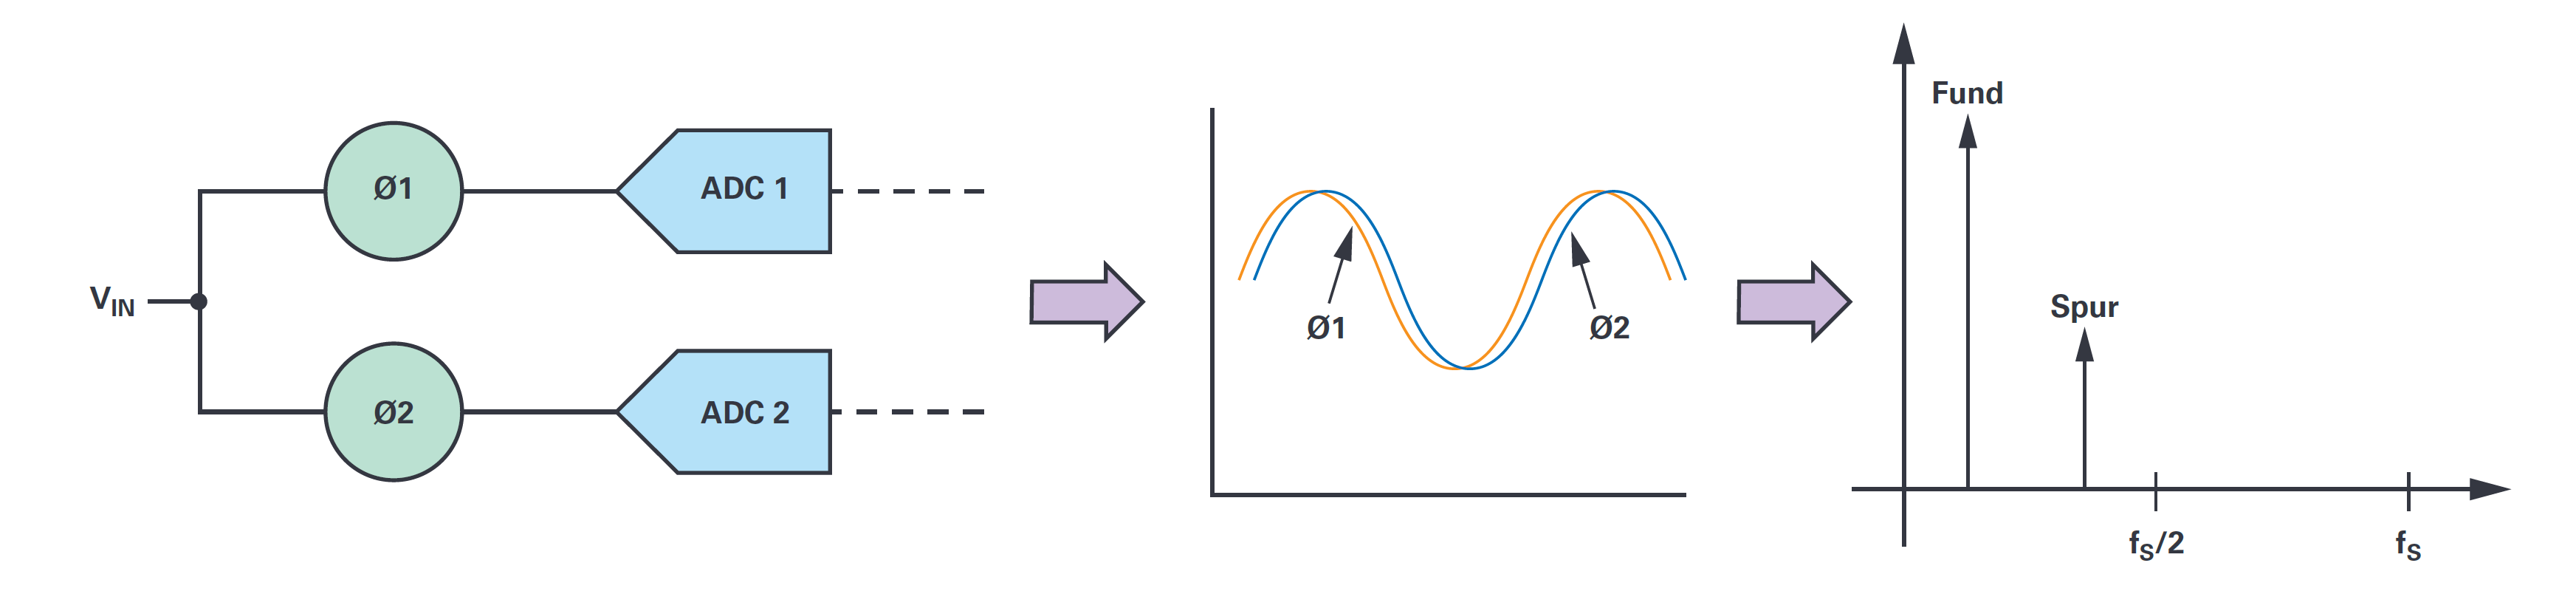
\includegraphics[width = \textwidth]{chap/02-theory/img/timing_mm}
	\caption{Placeholder: Timing-Mismatch in Interleaving \cite{Harris2019}}
	\label{fig:timing_mm}
\end{figure}

The last possible mismatch is the \textit{bandwidth mismatch}, which contains both gain and phase/frequency component (see \autoref{fig:bandwidth_mm}). Due to bandwidth mismatch, different gain values at different frequencies can be seen. An additional timing component causes different delays for signals at different frequencies through each \gls{adc}. Just like gain and timing mismatch, the bandwidth mismatch causes a spur at $f_s/2 \pm f_{\text{in}}$.
\begin{figure}[tbh]
	\centering
	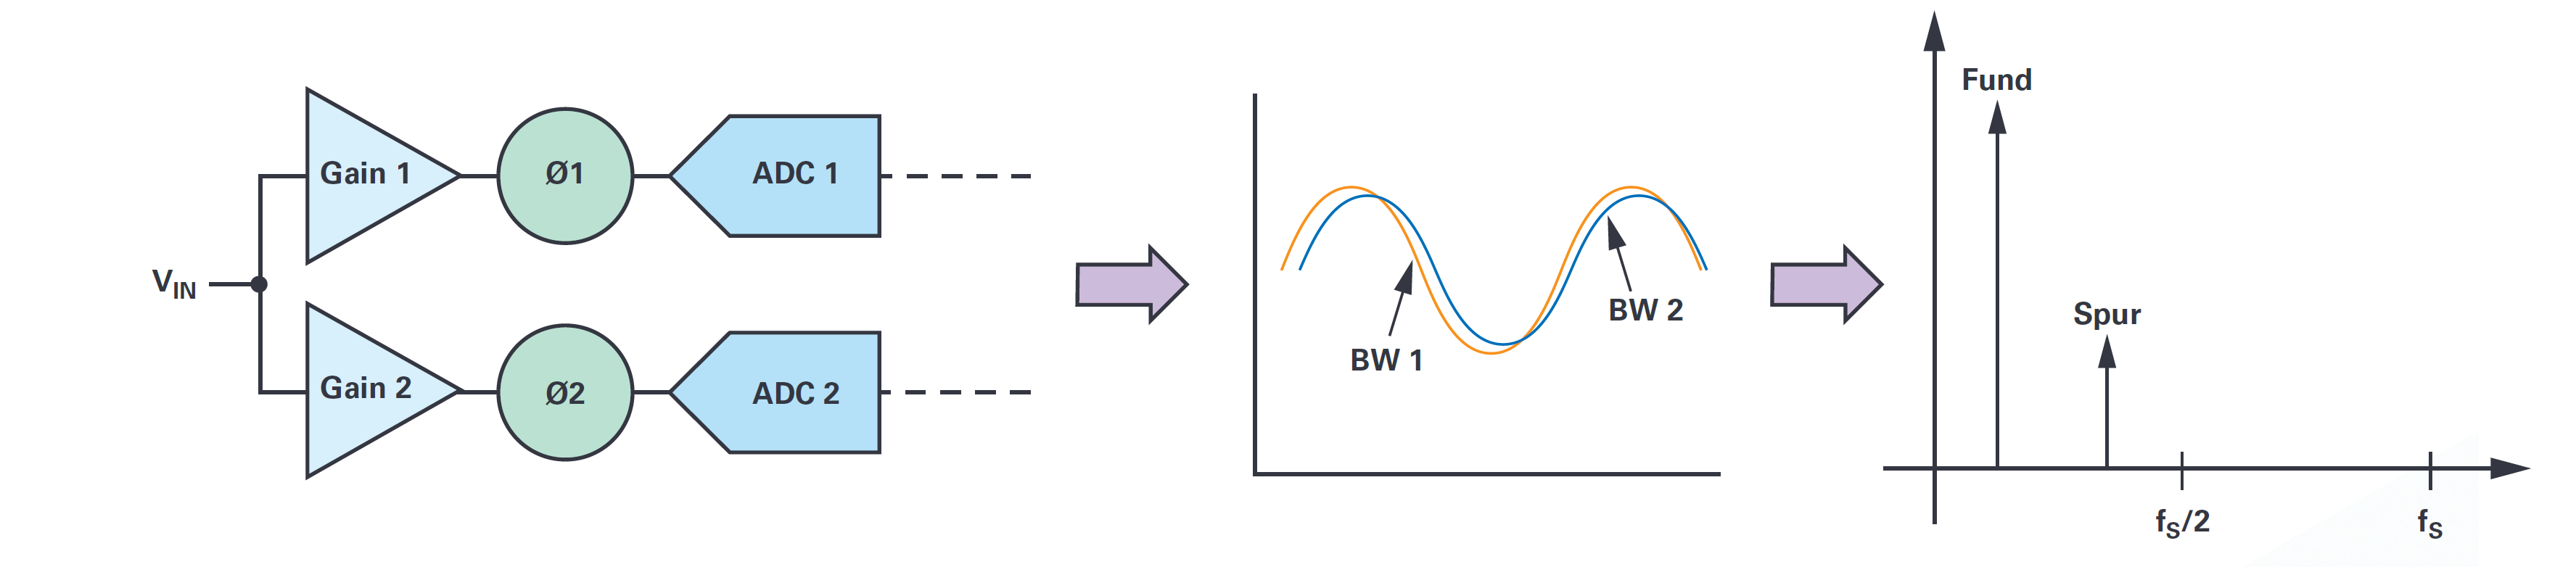
\includegraphics[width = \textwidth]{chap/02-theory/img/bandwidth_mm}
	\caption{Placeholder: Timing-Mismatch in Interleaving \cite{Harris2019}}
	\label{fig:bandwidth_mm}
\end{figure}